%\documentclass[11pt]{report}
\documentclass[a4paper,11pt,twoside,onecolumn,openright]{memoir}
\usepackage{geometry}
\geometry{a4paper}
%\usepackage[parfill]{parskip}%Activate to begin paragraphs with an empty line rather than an indent
\usepackage[pdftex]{graphicx}
\usepackage{amssymb}
\usepackage{epstopdf}
\usepackage{natbib}
%\usepackage{ltxfront}
\usepackage{tocvsec2}
\usepackage[hang,footnotesize,bf]{caption}
\usepackage[pdftex,bookmarks=true]{hyperref}
\usepackage{enumerate}
\bibpunct{[}{]}{;}{a}{}{,}
\DeclareGraphicsRule{.tif}{png}{.png}{`convert #1 `dirname #1`/`basename #1 .tif`.png}
\setcounter{secnumdepth}{2}

%Interacting with Smartphones on Tabletop Computers
%Combining Smartphones and Tabletops: Interaction Design

\title{\Huge TIDE: Using Device Composition on Tabletop Computers to Extend the Smartphone Experience.}
\author{\textbf{Master Thesis}\\by\\Leo Sicard\\(lnsi@itu.dk)\\
\\
\textbf{Supervisor:}\\Professor Jakob E Bardram\\
\\}
\date{March 1st, 2012\\IT University of Copenhagen, Denmark}

\begin{document}

%\maketitle
%\begin{figure}[h!]
%  \centering
%    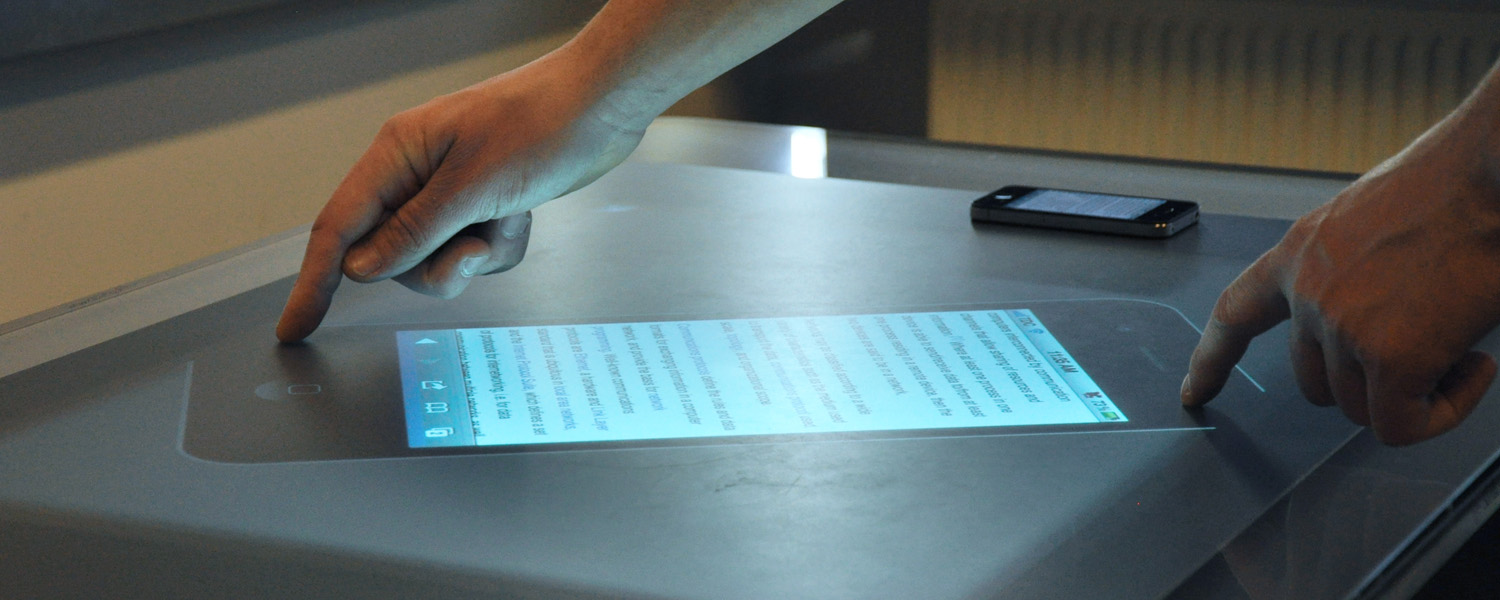
\includegraphics[width=0.8\textwidth]{images/tide314}
%\end{figure}
%\clearpage

\pagestyle{empty}

\begin{centering}
\hfill\\
\hfill\\
\hfill\\
\hfill\\

\Huge TIDE: Using Device Composition on Tabletop Computers to Extend the Smartphone Experience.
\hfill\\
\hfill\\
\begin{figure}[h!]
  \centering
    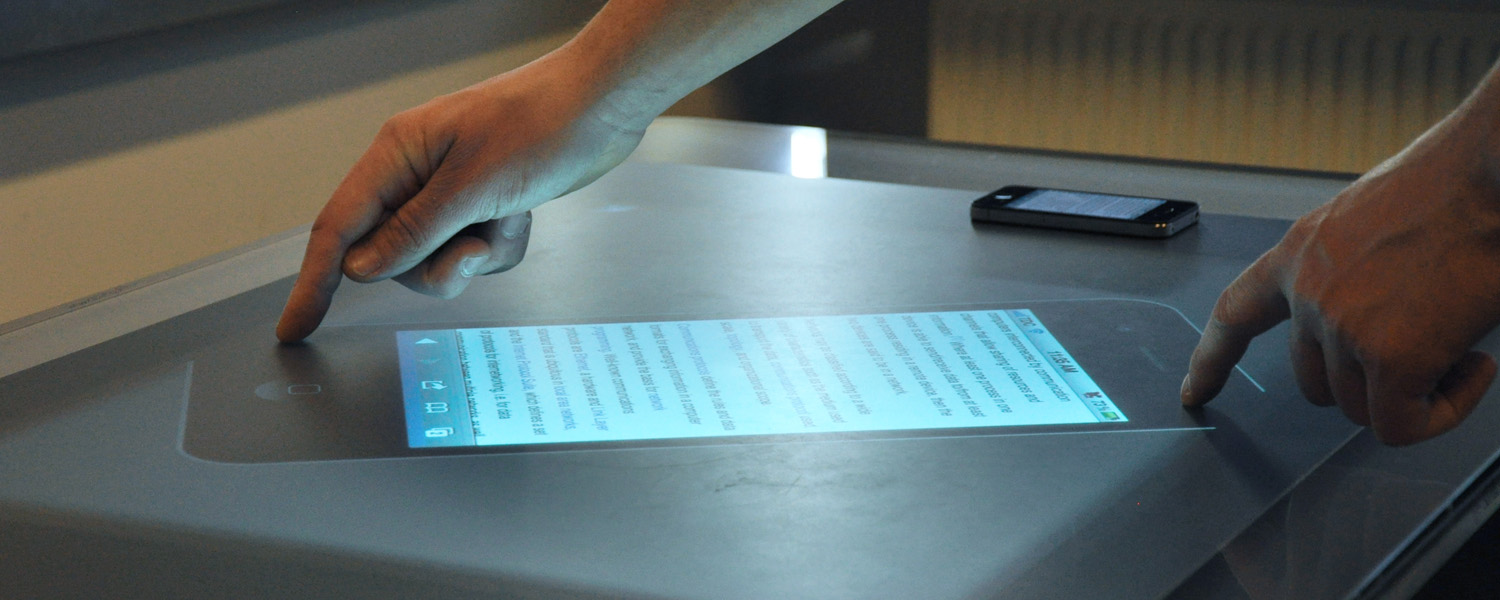
\includegraphics[width=0.8\textwidth]{images/tide314}
\end{figure}
\large
\hfill\\
\hfill\\
\textbf{Master Thesis}\\by\\Leo Sicard\\
\emph{lnsi@itu.dk}\\
\hfill\\
\hfill\\
\textbf{Supervisor:}\\Professor Jakob E Bardram\\
\hfill\\
\hfill\\
\hfill\\
\hfill\\
\hfill\\
\hfill\\
March 1st, 2012\\IT University of Copenhagen, Denmark\\
\end{centering}
\clearpage

\newpage
\hfill\\
\hfill\\
\hfill\\
\hfill\\
\hfill\\
\hfill\\
\hfill\\
\hfill\\
\hfill\\
\hfill\\
\hfill\\
\hfill\\
\hfill\\
\hfill\\
\hfill\\
\hfill\\
\hfill\\
\hfill\\
\hfill\\
\hfill\\
\hfill\\
\hfill\\
\hfill\\
\hfill\\
\hfill\\
\hfill\\
\hfill\\
\hfill\\
\hfill\\
\hfill\\
\hfill\\
\hfill\\
\hfill\\
\hfill\\
\hfill\\
\hfill\\
\linebreak
IT University of Copenhagen\\
Rued Langgaards Vej 7, DK-2300 K\o benhavn S, Denmark\\
Phone +45 72185000\\
itu@itu.dk\\
www.itu.dk\\
%\mbox{}
\clearpage

\hfill\\
\hfill\\
\hfill\\
\hfill\\
\hfill\\
\hfill\\
\hfill\\
\hfill\\
\hfill\\
\hfill\\

\begin{abstract}
Tabletop displays are now appearing in public spaces.
They present a horizontal interactive surface that is ideal in social situations, and they support a touch-based experience which appeals to all users.
Modern smartphones are able to support most users' daily computing tasks, and their mobility bring spontaneity to the computer interaction.
However, the screen size of smartphones is a limitation when viewing graphically intense content and in situations with multiple users.

This thesis focuses on extending the smartphone experience to tabletop displays.
It investigates the use of \emph{device composition} to allow smartphone users to spontaneously annex the display space made available by tabletops.
In particular, this report presents the design, implementation and evaluation of \emph{TIDE (Tabletop Interactive Display Extension)}; a composite device that integrates a smartphone to a tabletop by way of UI replication, with focus on \emph{spontaneous user interaction}.

The design process shows that by following a human-centered approach and using interaction techniques that are familiar to most users, the system can be designed to be easy to learn and easy to use.
The implementation of TIDE demonstrates that it is feasible to build this type of system on standard hardware and standard platforms.
Moreover, TIDE supports multiple simultaneous smartphones, and uses computer vision to track the location of the devices on the display.
The evaluation of TIDE, in the form of a participant-based usability study, shows that the system is highly learnable, easy to use, and useful in context.
\end{abstract}

\clearpage

\newpage
\mbox{}
\clearpage

\hfill\\
\hfill\\
\hfill\\
\hfill\\
\hfill\\
\hfill\\
\hfill\\
\hfill\\
\hfill\\
\hfill\\

\renewcommand{\abstractname}{Acknowledgements}

\begin{abstract}
First and foremost, I would like to thank Professor Jakob E. Bardram, for supervising this project and teaching me how to write a thesis.

Next, I thank Dr. Juan David Hincapie-Ramos and Postdoc Aur\'{e}lien Tabard for their involvement as thesis advisors; for the precious council, continuous support, and for giving me confidence.
In particular, I thank Juan for the idea that initiated this thesis.

Then, I thank all the people who gracefully volunteered to participate in the user experiments.

Finally, I give my thanks to:
\tightlists
\begin{itemize}[-]

\item Sebastian B\"{u}ttrich and the PITLab (Pervasive Interaction Technology Lab) for providing the hardware and working space,

\item Mads Frost for taking and fixing pictures,

\item Marie Choe Tarp for drawing,

\item Ane Tarp and Jakob Borg for proofreading,

\item the researchers and students associated with the PITLab for the support and helpful comments.

\end{itemize}
\end{abstract}

\clearpage

\newpage
\mbox{}
\clearpage

\pagenumbering{arabic}
\pagestyle{headings}
\maxtocdepth{section}
\tableofcontents
%\listoffigures

\clearpage

\firmlists



%%%%%%%%%%%%%%%%%%%%
%%% INTRODUCTION %%%
%%%%%%%%%%%%%%%%%%%%

%PROBLEM : WHICH INTERACTION TECHNIQUES TO USE WHEN DEVELOPING FOR UI REPLICATION BETWEEN A SMARTPHONE AND A TABLETOP?
%
%SOLUTION : THE PROTOTYPE, SUPPORTED BY BOTH STUDIES

\chapter{Introduction}
\label{introduction}

\begin{figure}[b!]
  \centering
    \includegraphics[width=0.6\textwidth]{images/tide3P}
  \caption{People viewing information on a smartphone.}
  \label{tide}
\end{figure}

\section{Background and motivation}

Modern smartphones are able to support most users' daily computing tasks.
They fit in a pocket, which makes them ultra mobile, and they offer good storage capacities as well as all-around connectivity.
This tendency implies that users have access to personal data and applications at all times.
Smartphones give rise to a new type of computer interaction which is unplanned, spontaneous, on-the-go.
They bring computing to situations where laptops don't fit, such as standing in a crowded train, or walking in the street.
Furthermore, they make it possible to get the most out of unforeseen opportunities, and in particular, they seem to be the ideal tool to support these chance meetings that suddenly turn into constructive collaboration.
However, the size of the device can be a limitation to this form of improvised computer interaction, especially in situations with simultaneous users. 
\\\\
Tabletop computers, on the other hand, are ideal in social contexts.
They bring computing to a very common piece of furniture, the table.
As such, they present a horizontal interactive surface around which multiple users can regroup, to share a common experience, or to conduct parallel activities.
They have been used extensively in museums and galleries, as documented by \cite{Geller:2006:exhibits}, who notes that tabletops encourage a collaborative atmosphere, and that they provide a tactile experience that reaches even the less computer literate.
Tabletops provide a touch-based experience that is fundamentally different from the traditional desktop metaphor.
A number of HCI studies show that this experience is a more natural one for the non-technical user, because it removes the mouse-and-keyboard abstraction layer and generates a more direct interaction.

\begin{figure}[htb]
  \centering
    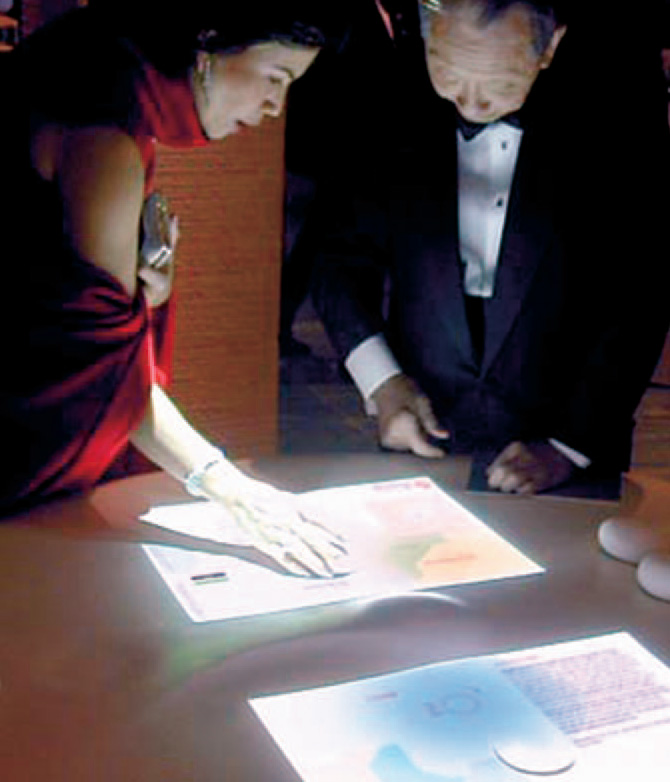
\includegraphics[width=0.4\textwidth]{images/visitors}
  \caption{People using an interactive tabletop\\exhibit at the Asia Society Museum.}
  \label{visitors}
\end{figure}

The first interactive tabletop displays were designed for individual use.
Systems such as the DigitalDesk \citep{Wellner:1993:digitaldesk} aimed at incarnating the desktop metaphor of the personal computer to the common office desk.
But tabletops have a huge potential for collaboration.
In following years, a research branch emerged that focused on \emph{smart rooms}: spaces equipped with various cutting-edge computing devices that can interoperate, to support collaborative work for multiple users.
Tabletops are an essential element of smart rooms, as shown with the InteracTable \citep{Streitz:1999:iland} and the iTable \citep{Johanson:2002:iroom}.

With the emergence of commercial items such as the Microsoft Surface \citeyearpar{ms}, tabletops are gradually appearing in public environments such as museums, meeting rooms, public lobbies, bars, restaurants, etc.
They are an ideal platform for spontaneous use and multi-user interactions, and they provide a touch-based experience that is similar than the one on most smartphones, making them easily accessible to the pubic.\\
\linebreak
%%% TECHNICAL REVIEW %%%%
%were based on overhead projected output and overhead camera-based input.
%In recent years, however, interactive displays are being commercialized, that are typically based either on computer vision or capacitance.
%
%Capacitive screens are present on the mass market since the iPhone \citep{iphone}, but are now being produced in larger sizes \citep{displax}, \citep{3m}.
%They function by sensing the electrical charge that is produced when a finger interacts with the screen's electrical field.
%This allow for a very precise touch detection, but a drawback is that it does not work with gloved fingers, digital pens or any other objects.
%
%Computer vision can be used in various ways.
%The first Microsoft Surface \citep{ms} as well as the MultiTaction displays \citep{multitouch} function with cameras that detect reflected infrared backlight from objects that are in contact with the screen.
%The main advantage of such solutions is that they can detect not only fingers, but also visual markers and other objects.
%Microsoft has perfected this technology in the latest Surface with PixelSense \citep{pixelsense}, where the individual pixels can detect what touches the screen, thus removing the need for cameras.
%PQ Labs \citep{pq} produces side vision overlays that can provide multi-touch detection to any type of screen, though without the possibility for object detection.

State-of-the-art smartphones boast screen resolutions up to 1280 by 720 pixels, that exceed the naked eye's ability to distinguish separate pixels.
%This implies beautiful graphics with profound and rich colors.
However, a smartphone screen is too small to provide a satisfying user experience in the presence of multiple users, and when viewing dense content such as text or high-quality images.
Screen sizes for ultra mobile devices go only up to 5 inches.
Reading a text, consulting a map and viewing images are examples of situations in which small displays present limitations.

An example of graphically dense content is a text of more than a few paragraphs.
The default view of an online blog or a pdf document on a smartphone is too small for a user to be able to discern single words.
Depending on one's eyesight, it usually takes 2 to 4 zooming gestures to enlarge the text to a size that is conveniently readable.
At this point, the user generally tilts the phone to a landscape orientation, to give the paragraphs a more natural length.
There is only space for 5 to 10 lines of text on the screen, which implies that the user uses successive pan gestures to update the content as s/he reads.
Compared to the casual experience of reading a newspaper article or a book, this seems like a lot of trouble.

Maps are also graphically dense.
They present a lot of different informations, such as topography, street names and sights, on limited space.
To be able to read a street name on a smartphone maps application, the user needs to zoom in on the relevant part of the map.
The result is that the user can only view a very limited area.
To be able to relate this area to, for example, his/her own location, the user must use a combination of pan and zoom out gestures that can be cumbersome.
In certain cases, the area of interest is simply too vast to be viewed on a smartphone screen.

Modern smartphones play the role of point-and-shoot cameras, due to the fact that we carry them with us at all times, and that they take pictures of high quality.
However, image viewing on a handheld device presents serious limitations.
Beside the fact that the screen is too small to do pictures justice, it makes showing them to someone else a frustrating experience.
Ideally, showing pictures to a friend implies both persons looking at the pictures together, to allow for commenting.
This is hardly possible with a smartphone.
A typical scenario is that the user finds a picture that he wants to show, then hands his phone to the friend, then the friend hands the phone back to the user, who chooses the next picture, and so on.
This process is cumbersome, and another example of the need for smartphones to be able to integrate with larger displays such as tabletops.

In the above mentioned cases, the smartphone provides all the necessary resources, with the exception of a large enough display.
This work focuses on these situations in which the smartphone experience would benefit from additional screen space.
\\
\linebreak
%It does so by suggesting a \emph{device composition} approach, that integrates smartphones and tabletops.
%Tabletops are a solution to this problem for several reasons.
%They provide the needed display space, and a touch-based interaction that comes naturally to the typical smartphone user.
%Moreover, they are designed for collocated collaboration, which brings an interesting new dimension to the scenarios discussed above.
%Examples of the possibilities include consulting a map to show a location to a friend, reading and editing a document with a colleague, playing a multiplayer game, or viewing and sharing pictures between smartphones.
A way to address this challenge is by using \emph{device composition}, a research approach that can be traced back to the work on smart space technologies and systems such as Augmented Surfaces \citep{Rekimoto:1999:augmentedsurfaces}, \mbox{i-LAND} \citep{Streitz:1999:iland} and the Interactive Workspaces \citep{Johanson:2002:iroom}.
Smart rooms were designed as closed computing environments, so recent efforts have been invested in developing for a more ad-hoc type of device composition, with projects such as Obje \citep{Edwards:2009:obje}, Platform Composition \citep{Pering:2009:platformcomp} and CompUTE \citep{Bardram:2010:compute}.

Tabletops are a central device in the aforementioned smart rooms, and a recurring element within device composition.
They are an ideal platform for collocated collaboration, as was shown with systems such as the MemTable \citep{Hunter:2011:memtable} and SketchTop \citep{Clifton:2010:sketchtop}, that are designed to support the work of technical users.
In recent years, however, tabletops are appearing in public spaces, aiming at engaging common users in a more casual form of interaction.
\\
\linebreak
Within this context, designing for device composition between smartphones and tabletops implies addressing three fundamental challenges.

The first one is the pairing procedure responsible for device discovery and connection.
Pairing between unknown devices has been solved in many different ways.
An example that is particularly relevant to this work is the BlueTable \citep{Wilson:2007:bluetable}, an interactive surface that uses Bluetooth to discover and connect to a mobile phone, but improves this process by using computer vision to locate the phone on the table, and verify its identity via the phone blinking an infrared signal.

The second challenge is how to distribute the UI of the smartphone to the tabletop.
There exists various stable technologies to choose from, but recent research works have chosen to build frameworks from scratch, to allow a more flexible distribution and sharing of user interfaces between multiple types of devices.
An example of such an approach is XICE (eXtending Interactive Computing Everywhere) \citep{Arthur:2011:xice}, a programming framework that is destined to support a new form of nomadic experience, where users can annex various display servers with their mobile personal devices.

The last challenge is to design a user interaction that suits the purpose of the system.
Different interaction metaphors have been used to extend the UI of smartphones to larger display surfaces, including streaming, replication, expansion, projection and adaptation.
In their recent work on Virtual Projection (VP), \cite{Baur:2012:virtualprojection} built a system where a smartphone can be used to seemingly project its UI onto an available computer display.

%Device composition started with SMART ROOMS, and composing various devices, which we want to do in this case.
%But smart rooms were designed as closed environments.
%
%We would like AD-HOC, spontaneous device composition.
%That was addressed by projects like Obje, CompUTE, Platform Composition.
%
%we are interested in mobile to TABLETOP
%- studies on collaboration (but closed environments and technical users)
%- studies on tangible interaction
%
%tabletops emerge in public spaces > non technical users > we focus on standard hardware
%
%we must solve 3 challenges: pairing, UI distributing, user interaction
%
%To combine SP and TT, we need to pair them, which can be done
%with networked protocols or bluetooth
%(but that requires explicit input from user, or CPU/battery intensive continuous sniffing
%SO we use a trigger, that can be:)
%detecting synchronous events
%entering a key into display
%with RFID
%with computer vision to detect
%
%we do it with computer vision detection and networked protocol (Bonjour)
%
%we need a technology to do UI distribution:
%distr data
%distr code
%
%best to distr graphics:
%(we choose VNC in spite of drawbacks > why?)
%
%we need a user interaction
%
%FINISH with how we do differently!

\section{Problem statement}

This thesis addresses the problem of using \emph{consistent} design to build a composite device between a smartphone and a tabletop computer, that allows for \emph{spontaneous interaction}.
\\
\linebreak
It does so by answering the following research questions:
\begin{itemize}
\item What are the requirements for such a system?
\item Which interaction techniques are best suited to this type of system?
\item Can this system be made to run on standard hardware and integrate different smartphone types?
\end{itemize}

\section{Research methods}

To solve the problem at hand, the following research methods were used.
\\
\linebreak
To place the present work within its research context, 
a comprehensive literary review was made of the prior work related to device composition and surface computing.
In particular, the following aspects of device composition were investigated: main approaches, tabletop systems and applications, pairing, UI distribution, user interaction.
The resulting study is presented in Chapter~\ref{relatedwork}.

Following a user-centered approach, a solution design was completed.
The process was divided into to the following tasks.
The application's context of use was analyzed with the support of scenarios and storyboards, which lead to the definition of solution requirements.
A series of design options were generated from the study of existing approaches to software design for surface computing.
With the support of a study based on low-fidelity prototypes and the involvement of potential users, a final design was produced.
The design process is reported in Chapter~\ref{design}

In order to demonstrate the feasibility of the suggested solution, a proof of concept was realized, in the form of an application prototype implemented on the Microsoft Surface tabletop computer, an iPhone 4 and a HTC Legend phone.
The implementation was focused on the user interaction, in the aim of showing that consistent design can lead to an easy user experience.
The system is described in Chapter~\ref{system}.

%Third-party applications are used on the smartphones, that requires rooting the devices.
%On the tabletop computer, the application is programmed within the .NET framework,  using specifically WPF (Windows Presentation Foundations) and the Presentation layer of the Microsoft Surface API 1.0.

An evaluation of the design was conducted by way of a usability study, that involved the following steps.
The focus of the evaluation was identified, in terms of specific aspects of the system, and the evaluation methods were selected.
A user experiment was designed, that involved a discovery phase, cooperative evaluation, a semi-controlled test and a questionnaire.
Participants were recruited, and the experiment was carried out.
Evaluation data was gathered via online forms as well as application logging.
The resulting data was processed, analyzed, and the evaluation results were derived.
The evaluation process and results are presented in reported in Chapter~\ref{evaluation}.

\section{Contributions}

This work consists of the design, implementation and evaluation of a composite device that integrates smartphones to the Microsoft Surface.
There are three major contributions.

\begin{enumerate}

\item The user-centered design process shows that it is feasible to design a system that is immediately accessible to all types of users, and that the user interaction plays an essential role in the design of an intuitive device.
To support the process of selecting the most intuitive interaction techniques, this work introduces two design principles: \emph{consistency} and \emph{physicality}.
The consistency of the design refers to the selection of interaction techniques that users already know from any type of prior experience.
The physicality of the design implies taking into consideration the form factor of the devices, to identify interaction techniques that are natural to the user.
%The tabletop interaction should be consistent with the smartphone interaction, reacting whenever possible as the user would expect a smartphone to.
%Well-known interaction techniques, such as the double tap, are easy for the user to discover, and can therefore be used accordingly.
%The physical form of the devices has implications on the user's expectations, that the interaction should be consistent with.
%Some implications can be translated to the design, such as the common expectation that moving a document off a table takes the focus away from it.

\item The implementation of the proof-of-concept application called \emph{TIDE (Tabletop Interactive Display Extension)} shows that it is feasible to implement a system on the Microsoft Surface (first generation) that allows users to integrate any type of smartphone to the tabletop by way of UI replication.
%It shows that the pairing procedure can be made quick and easy by using camera-based object detection and wireless connectivity.
%The display of the smartphone is replicated to the tabletop, and is referred to as the \emph{remote UI}, allowing the user to interact with his phone indirectly.
%The remote UI is contained in an application window that is referred to as the \emph{surface UI}, whose role is to allow for the manipulation of the remote UI on the tabletop display.
%The UI replication is based on the VNC protocol \citep{Richardson:1998:vnc}.
%Currently supported devices are iOS and Android smartphones, but TIDE can be extended to support other devices.

\item The final contribution is the evaluation of the application design.
It shows that consistency and physicality allow the design of a device that is easy to use for all types of users.
Furthermore, it shows that it is a good idea to implement several interaction techniques for a same feature, in order to reach users with different background.
Finally, the evaluation confirms that there is a need for a system that allows users to extend their smartphone screen space to a larger display.

\end{enumerate}

%\section{Thesis overview}
%
%Chapter~\ref{relatedwork} presents a literary review of the research that constitutes the background to this work, and the theoretical work on which the design approach is based.\\
%Chapter~\ref{design} describes the process that lead to the design of the TIDE prototype.\\
%The system itself is presented in Chapter~\ref{system}, and its evaluation by way of a usability study in Chapter~\ref{evaluation}.\\
%Chapter~\ref{discussion} is a discussion that addresses the results and lessons learned throughout this process, and brings suggestions for future work.\\
%Chapter~\ref{conclusion} concludes the report.

% solution : using tabletops as UI peripherals
%%%%%%%%%%%%%%%%%%%%%%%%%%%%%%%%%%%%%%
%The specificity of tabletops raises the question of how to interact with them on an everyday basis.
%Recent development initiatives tend to answer this question by regarding tabletops as yet another computational platform, requiring its own software.
%With this project, we explore a different approach to integrating tabletops in our environment, namely by using them only as UI peripheral, providing touch-based input and graphical output to the devices that we already have.
%Exploring this path is supported by three important factors.
%First, most users already own computing devices, such as laptops or smart phones, with tailor-made applications and local storage, and might be less prone to use an additional device if it requires management (updates, backups, synchronizations, etc) and the purchase of applications.
%Second, tabletops are embedded in the environment and as such can be expected to be shared devices.
%Using them as simple graphic peripheral would allow to avoid the traditional desktop/laptop issues related to user profiles, privacy and data integrity.
%Finally, as embedded devices, it is reasonable to expect tabletops to have good networking capabilities.

% device composition
%%%%%%%%%%%%%%%%%%%%%%%%%%%%%%%%%%%%%%
%Device composition focuses on getting the most out of various computing entities, by making them work together and function as one, as seen in \cite{Bardram:2010:compute}.
%This project explores device composition for UI integration between tabletops and mobile devices, focusing on seamless user experience and implicit human computer interaction as defined by Schmidt in \cite{Schmidt:2000:implicit}.

% UI integration metaphors
%%%%%%%%%%%%%%%%%%%%%%%%%%%%%%%%%%%%%%
%UI integration can happen in several different ways:
%\begin{itemize}
%\item{\emph{UI transfer} (mirror): the tabletop `takes over' and displays the UI of the connected device.}
%\item{\emph{Dual view}: the tabletop display becomes secondary screen space for the connected device.}
%\item{\emph{UI nesting}: the connected device is physically located on the tabletop, and its UI is extended to the additional screen space around it.}
%\end{itemize}

% challenges
%%%%%%%%%%%%%%%%%%%%%%%%%%%%%%%%%%%%%%
%Following is an open list of problems that we will address in order to achieve device composition by means of implicit interaction.
%\begin{enumerate}
%\item{\emph{Setup}: How is a device enabled for integrating with a tabletop?
%The setup should be simple, to be performed only once by non-technical users.
%An initial survey of possible solutions points towards the use of tagging mechanisms and/or camera-based object recognition.}
%\item{\emph{Discovery}: How do the tabletop and the device discover and communicate with each other?
%How do we solve the issues of discovery, handshake, network connectivity, and encryption mechanisms to ensure privacy?}
%\item{\emph{UI transfer}: Given the computational constraints of mobile devices, how can the UI transfer be efficiently implemented so as to support native applications and guarantee a seamless user experience?}
%\item{\emph{Input}: How can the users interact with their applications on the tabletop (touch and other peripherals)?}
%\item{\emph{Interaction Design}: What means of interaction are best-fitted for the tabletop-based systems that we propose to develop?
%How can we best adapt to public/private uses and single/multiple users?
%How can we take advantage of the larger interaction surface?}
%\end{enumerate}


\chapter{Related Work}
\label{relatedwork}

%Due to their relevance to the current project, the following aspects of device composition are reviewed: smart spaces, pairing, UI distribution and tabletops.
%Lastly, the main approaches to designing user interaction for device composition between mobile devices and larger displays are presented.

%\subsubsection{Device composition}

%DEVICE COMPOSITION is an approach that can solve this.
%%%%%%%%%%%%%%%%%%%%%%%%%%%%%%%%%%%%%%%%%%%%%%%%%%%%%%%%%%%%%%%%%%%
\emph{Device composition} is an important element of the ubiquitous computing research area, and the main background of this thesis.
An essential aspect of ubiquitous computing is the idea that users can benefit freely from the resources that are available in the environment.
%Device composition started with SMART ROOMS, and composing various devices, which we want to do in this case.
%But smart rooms were designed as closed environments.
%%%%%%%%%%%%%%%%%%%%%%%%%%%%%%%%%%%%%%%%%%%%%%%%%%%%%%%%%%%%%%%%%%%
Extensive research focused on realizing that idea by designing computer augmented spaces, or \emph{smart rooms}, where heterogeneous devices can interoperate.
Examples of such smart spaces are Augmented Surfaces \citep{Rekimoto:1999:augmentedsurfaces}, 
%where portable devices and interactive surfaces are enabled for data exchange; 
i-LAND \citep{Streitz:1999:iland} and the Interactive Workspaces \citep{Johanson:2002:iroom}.
Beside device interaction, these projects were aimed at supporting collaborative work between collocated users.
Smart rooms are usually closed computing environments that rely on a centralized software infrastructure, such as BEACH developed for i-LAND \citep{Tandler:2001:smartenv}, or Gaia OS for Active Spaces \citep{Roman:2002:gaia}.
The advantage of such an approach is that the interaction between the enabled devices can be hugely optimized, as they shared a set of semantics.
However, the drawback is that new devices cannot be integrated easily, requiring at least a software installation or configuration.

%We would like AD-HOC, spontaneous device composition.
%That was addressed by projects like Obje, CompUTE, Platform Composition.
%%%%%%%%%%%%%%%%%%%%%%%%%%%%%%%%%%%%%%%%%%%%%%%%%%%%%%%%%%%%%%%%%%%
To bring device composition outside of the smart rooms, systems have been built, that support a more ad-hoc form of device interaction.
Obje \citep{Edwards:2009:obje} is a middleware that relies on services transferring mobile code to achieve device compatibility at runtime.
It allows devices to interoperate upon their very first encounter, but relies on the user's semantic interpretation to do so.
\cite{Pering:2009:platformcomp} focused on understanding ad-hoc collaboration using pervasive technologies, and suggested Platform Composition as a technique to support collaborative work by using a combination of standard computing components.
\cite{Bardram:2010:compute} developed CompUTE, a runtime architecture for device composition  on Windows XP systems based on the extended desktop metaphor.
\\
\linebreak
% END WITH TABLETOP
\emph{Tabletop displays} are an recurring element in research projects that address device composition.
They present two important characteristics.
First, they are \emph{situated}, i.e.\ due to their size, they typically sit in a location and are not moved frequently.
Second, they are \emph{shared} among multiple users, mostly due to their horizontal interactive surfaces that allow users to attend from all angles and engage in face-to-face interaction.
For these reasons, tabletops seem to be best used in combination with the mobile devices carried around by users, especially when they sit in a public space.

Even though early systems such as the DigitalDesk \citep{Wellner:1993:digitaldesk} were designed for the individual office desk, most of the research on tabletops has been focused on their potential as support for collocated collaboration.
Thanks to technology advances such as DiamondTouch \citep{Dietz:2001:diamondtouch},
% that combines overhead projected output with capacitively sensed input,
tabletops support multiple simultaneous touch input, and thus simultaneous users.
They are an essential element of smart spaces, with systems such as the InteracTable for the i-LAND \citep{Streitz:1999:iland} and the iTable for the iRoom \citep{Johanson:2002:iroom}.
Other projects have shown that they are an ideal tool to support collaboration, with systems such as the MemTable \citep{Hunter:2011:memtable}, that permits the capture and recall of meetings, or SketchTop \citep{Clifton:2010:sketchtop}, a multitouch sketching application for collocated design collaboration.

Another basic characteristic of tabletops is the horizontal orientation of their interactive surface.
The obvious implication is that physical objects can be placed on them.
Much work has gone into the detection and tracking of such objects, with systems such as SurfaceFusion \citep{Olwal:2008:surfacefusion}, where the authors used a combination of RFID technology to sense the presence of objects and computer vision to track their precise location.
Tracking techniques can be used to detect other computing devices, and can therefore help to solve certain challenges of device composition.

% tangible interaction %
%The integration of innate objects to tabletop systems has given rise to a research branch called \emph{tangible interaction} ..
%
%There is basically two ways to integrate physical objects to interactive surface.
%The first one is to use the objects as a tangible user interface (TUI), a notion that was introduced with the MetaDESK \citep{Ullmer:1997:metadesk}.
%The second approach has for purpose to augment objects with digital information.
%Examples of this approach include SurfaceWare \citep{Dietz:2009:surfaceware}, which allows the Microsoft Surface to sense the fluid level in a slightly enhanced drinking glass, and the Rabbit \citep{Hincapie:2011:rabbit}, a device that integrates small RFID-tagged objects and tabletops.

In recent years, tabletops are being commercialized, and gradually appear in public spaces such as firm lobbies, shops, bars and restaurants.
For example, the Microsoft Surface is part of the furniture in the new retail stores of the Royal Bank of Canada \citep{mscase}, offering service applications to the visiting customers.
This tendency gives rise to a new type of tabletop interaction, more spontaneous, and targeting non technical users.
It is within this context that the present work is set.

The task of the present work is to design a composite device made up of a smartphone and a tabletop for spontaneous user interaction.
This task poses three fundamental challenges: device pairing, distributing the user interface and designing the user interaction.

\subsubsection{Pairing}

\emph{Pairing} is an essential part of any device composition, and a challenge that can be solved in many ways.
Some systems are designed for networked devices, and achieve pairing with TCP/IP based networking protocols such as Zeroconf \citeyearpar{zeroconf} for Obje and UPnP \citeyearpar{upnp} for CompUTE.

Bluetooth \citeyearpar{bluetooth} supports a device discovery protocol that was used by the Personal Server \citep{Want:2002:personalserver}.
It allows the pairing of any bluetooth-enabled device, but the process has been shown to be slow, and can be inefficient if there are multiple devices in the vicinity.

In systems that allow for spontaneous interaction between wireless mobile devices, additional techniques must be used to permit the identification of the correct device.
A way to do that is by detecting synchronous events, like with the Smart-its \citep{Holmquist:2001:smartits}, that connect when they are held and shaken together; and SyncTap \citep{Rekimoto:2003:synctap}, that requires the same key to be simultaneously pressed on both devices.

Another technique that has been used to connect mobile devices to a situated one, e.g.\ a large display, is to have the display present a random key to be entered on the mobile device.
The key can take the form of an alphanumeric string, a sequence of motions \citep{Patel:2004:mobileauth}, or a visual pattern \citep{Ballagas:2005:sweeppointshoot, Scott:2005:visualauth}.
This approach allows authentication, but adds steps to the pairing process.

Established RFID technologies can be used for device association, but requires that the mobile device is equipped with the appropriate tag, and that the situated device presents an RFID reader.
Upcoming NFC techniques present the great advantage that devices can function both as reader and transmitter, but few commercial devices are equipped as of yet.

Computer vision can be used to detect specific shapes, such as phone-like objects.
It can make the pairing process easier, as shown with the BlueTable \citep{Wilson:2007:bluetable}, an interactive surface that uses vision techniques and Bluetooth to pair with a mobile phone.
%\\
%\linebreak

\subsubsection{UI distribution}

Device composition has been extensively used for building systems that allow the distribution of user interfaces between devices.
The typical setup is to be able to view and interact with the data and applications from a mobile device on a situated one that offers superior display resources.
There are various technologies for UI distribution.

One way is to distribute only the data to the larger display, such as was done for the iRoom \citep{Johanson:2002:iroom}, but this approach is only applicable when both devices have the same software installed.

Another possibility is to distribute code, sending whole applications to the situated device for execution.
However, there are a series of issues with such an approach.
The situated device might not be able to run the application, either because of compatibility problems (hardware, software) or because the device might choose not to trust unknown code.
Software can be compiled into platform-independent code, such as is the case for Flash \citep{flash}, Java \citep{java} and Silverlight \citep{silverlight}.
However, issues remain, that are mostly related to the excessive size of the data files and the security risks.
\\
\linebreak
Distributing graphics is generally a preferred approach, because it allows to keep user data and credentials on the mobile device, and it has better potential for responsive interaction.
Systems such as X-Windows (X11) \citep{Scheifler:1986:x11}, Remote Desktop Protocol (RDP) \citep{Tritsch:2003:rdp} and Virtual Network Computing (VNC) \citep{Richardson:1998:vnc} utilize rendering-based protocols for UI distribution.
Applications are executed on a device, and rendered on another.
These protocols are stable, but they are based on the assumption that the machine executing the application has important resources.
When combining mobile and situated devices, however, the situation is reversed: the computer with the greater resources renders the graphics.

Another way of distributing graphics is by using web-based protocols, where Hypertext Transfer Protocol (HTTP) and Hypertext Mark-up Language (HTML) are used to send and present the application.
Such an approach can either be built on a web server model, which is basically what we use when we log on to websites via a browser, or on a personal server model, which is what the Personal Server \citep{Want:2002:personalserver} was based on.
The Personal Server is a handheld device without a display, that transmits HTML pages to available displays in the environment.
Using a web-based protocol implies a series of drawbacks that are induced by the use of HTML: browsers behave differently, HTML 1 to 4 does not support generalized drawing, HTML does not handle varying display sizes and resolutions and the use of Javascript introduces security issues related to programmable display.

Arthur and Olsen \citeyearpar{Arthur:2011:xice} address UI distribution with XICE (eXtending Interactive Computing Everywhere).
XICE is a programming framework that uses wireless networks to connect portable devices to display servers.
It takes into account the limited CPU and battery capacities of mobile devices, and provide a flexible protocol that allows the annexation of different types of displays.

Gjerlufsen et al.\ \citeyearpar{Gjerlufsen:2011:substance} have also taken the approach of building a framework to support the development of interactive multi-surface applications.
Substance is a data-oriented programming model that was used to build a middleware that provides powerful sharing applications.

%X-based window system to facilitate the design, implementation and evaluation of innovative window management techniques \citep{Chapuis:2005:metisse}.

% TRACKING USERS
%survey of advances in vision-based human motion capture and analysis between 2000 and 2006, show substantial progress with automatic human motion tracking and recognition.
%\citep{Moeslund:2006:motioncapture}

%Device composition has been steadily gaining importance due to the growing multiplicity of computing devices and mobility of users.
%Nowadays, a typical user owns mobile computers (handheld, tablet, laptop, etc\ldots) and interacts with other devices in an ad hoc way, as s/he comes upon them throughout the day (public desktops, printers, displays, etc\ldots).
%Enabling efficient communication and collaboration between various devices is therefore an essential issue, with the overall goal of improving the user experience.

%Device composition focuses on the following challenges:
%\begin{description}
%\item[Connection:] this includes device detection, identification and connection.
%\item[Communication:] different types of devices (hardware, OS) must use a common language if they are to collaborate.   
%\item[Sharing:] collaboration often requires sharing information. Besides technical problems, this raises the privacy issue of protecting the user's personal data.
%\item[Interaction:] the user must be able to interact with the system if s/he is to benefit from it.
%\end{description}
%\hfill\\
%This project focuses on the human computer interaction aspect of combining smartphones and tabletops.

\subsubsection{User interaction}

%- intro / theory = Norman, Buxton (sketching user experiences)
%- methods / approaches
%- gestures
%- interactions

Recent research efforts have been invested in combining mobile devices such as smartphones to different types of larger displays, such as tabletop computers.
The aim is always similar: extending the user interface of the phone to improve the user experience.
But different approaches are possible in terms of the interaction metaphor that the extension is based on.

\emph{Streaming} is a straightforward approach where only the visual output of the mobile device is forwarded to a remote display.
It is what happens when we connect a laptop to a projector, for example to give a presentation.
This is a satisfying solution in specific situations, and present the advantage of being secure, because input is kept to the mobile device.
However, it presents serious limitations in terms of interaction potential.

\emph{Replication} goes one step further, by allowing the user to provide input on the replicated UI.
This type of integration is already available for personal computers, but requires using a cable, or a docking station.

\emph{Expansion} is when the larger display is added to the UI of the mobile device.
It provides the possibility of transferring data or applications to the remote  machine, while keeping the mobile UI independent and available.

\emph{Projection} is a metaphor similar to replication, with the difference that the mobile device itself is used for projecting its UI onto an available display surface.
\cite{Winkler:2011:interactivephonecall} have built a device composed of a smartphone and a personal projector, that provide powerful in-call collaboration features, by projecting a shared interface on any available surface.
Virtual Projection (VP) \citep{Baur:2012:virtualprojection} is a system where a smartphone can be used to project its UI onto an available display.

\emph{Adaptation} refers to an improved UI transfer where the UI is modified to make full use of the additional resources available on the remote display.
This approach was followed by the authors of XICE \citep{Arthur:2011:xice}.



%\chapter{Theory}
%%%%%%%%%%%%%%
%%% DESIGN %%%
%%%%%%%%%%%%%%

\chapter{Design}
\label{design}

This chapter reports the design process for building a composite device that integrates smartphones with tabletops and provides a spontaneous user interaction.

A user-centered design approach was followed, in the purpose of understanding the system's context of use, and identifying the interaction techniques that would make for an intuitive application.
This process was supported by methodological tools described in Designing Interactive Systems \citep{Benyon:2010}.
Brainstorming, scenarios, storyboards and low-fidelity prototypes were used, and a study involving end users was carried out, the results of which informed the final design.

\begin{figure}[htb]
  \centering
    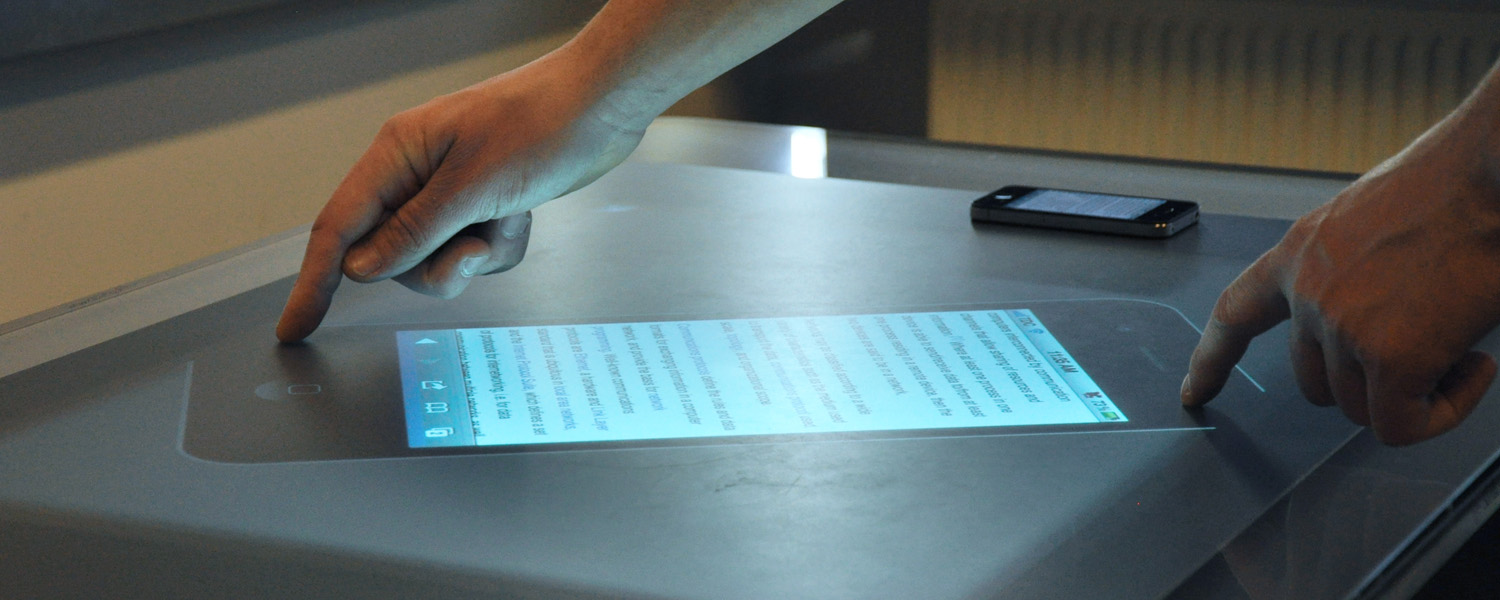
\includegraphics[width=0.8\textwidth]{images/tide314}
    \caption{The TIDE prototype.}
    \label{fig:tideHands}
\end{figure}

The focus of the design was on learnability and ease of use.
The goal was to build an intuitive system, i.e.\ a system that users understand without conscious reasoning.

To reach this goal, the design principle of conceptual consistency, as defined by \cite{Benyon:2010}, was used.
In this particular case, consistency was used in relation to two important aspects.
First; given that all the users of the system are smartphone users, the final system should provide a user experience that is as consistent as possible with the smartphone experience.
Second; the user interaction should be consistent with the implications that the devices' form have on the user's expectations.
In particular, the interaction should be consistent with the form of the table, e.g.\ various objects could be placed on the tabletop during an application session.
\\
\linebreak
It was decided to limit the focus of this work to one interaction metaphor: \emph{UI replication}.
This metaphor was chosen among the different possibilities enumerated in Chapter~\ref{relatedwork}, for the following reasons.
First, UI replication allows for a strong consistency between the experience on the smartphone and the experience on the tabletop.
Second, UI replication implies that the smartphone's application logic stays unchanged, and allows for the development effort to be focused on the tabletop.
Third, for the same reason as mentioned above, the implementation can be made to support different types of smartphones.

Thus, the system is designed to present the user with a mirrored image of the smartphone UI on the tabletop.
This is referred to as the \emph{replicated UI}.
It is interactive, relaying touch input and graphical output between the smartphone and the tabletop.
The replicated UI is controlled by the \emph{surface UI}.
The surface UI consists of elements that allow for manipulation of the replicated UI on the tabletop.
\\
\linebreak
An analysis of the context of use is presented in section~\ref{sec:context}, from which solution requirements are derived in section~\ref{sec:requirements}.
Section~\ref{sec:interaction} describes the generation of design options for the surface UI and their evaluation.
The final design of the TIDE prototype is presented in section~\ref{sec:design}.

\section{Understanding the application context}
\label{sec:context}

Some initial design constraints were already known; namely the system integrates smartphones with tabletops, and the system uses UI replication to extend the smartphone UI to the tabletop.
%Figure \ref{fig:useCase} describes the primary use case.
Additional design constraints were derived from an analysis of the devices, as well as an analysis of the context of use based on scenarios.

%\begin{figure}[htb]
%  \centering
%    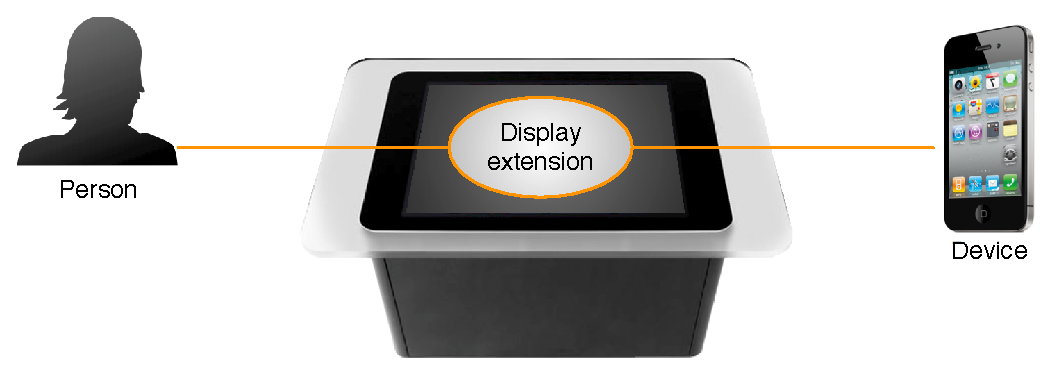
\includegraphics[width=0.9\textwidth]{images/useCase}
%    \caption{Main use case.}
%    \label{fig:useCase}
%\end{figure}

%Most users own a computing device with personal data and applications that are tailored to their needs.
%Those personal devices are becoming smaller and more mobile, with devices such as tablet and handheld computers.
%In many cases, the display size of the personal device is a limitation in terms of graphical input and output, and has a negative influence on the user experience.
%One of the main characteristics of tabletops, however, is that they have superior graphical I/O capabilities.
%This project focuses on situations where a tabletop can be used as a display extension to the personal device, thus enhancing the user experience.

\subsection{The devices}

The basic characteristics of the devices have concrete implications on the system design.

\subsubsection{A tabletop is\ldots}

\begin{description}

\item[\ldots a computer.]
The tabletop provides computing resources such as processing power, memory and connectivity; as well as an operating system that supports software applications.

\item[\ldots a table.] 
Its physical form comprises a horizontal surface that is commonly used to support various material objects.
A table is used for various activities, such as studying, eating, playing games, holding meetings, etc.
It can be approached from all angles, encouraging face-to-face interaction between multiple users.
%The system should therefore support simultaneous users, and handle limited space availability.

\item[\ldots a situated device.] 
It usually sits at a location, and is not moved often.
It can be expected to have dedicated power supply and network connection.
Users approach it to use it, and leave when they are finished.
Thus, the interaction flow is likely to be interrupted, taking the form of short successive sessions.
The nature of the location has an impact on the user interaction, and should be considered.
Examples are a conference room, a public lobby, a mall, an individual office, a living room in a family house, etc.
%The main implication is that tabletops seem to naturally fit in public spaces, where they are shared among multiple users.
%This tendency is accentuated by the price factor, that makes a private person not likely to buy such a device for private use.
%The system should handle public use, characterized by short anonymous sessions and an often interrupted interaction flow.

\item[\ldots a shared device.] 
When located in a public space, the tabletop is shared among multiple users.
Depending on the context and the relationship between the users (friends, colleagues, strangers, etc), the level of trust varies.

\item[\ldots an interactive surface.] 
It typically offers a large graphical output, and a range of input techniques that allow for user interaction.
Most tabletops support multitouch-based input.
%This introduces a new kind of interaction model, more intuitive, that the system should be based upon.
Some tabletop models support computer-vision techniques that allow for the integration of tangible objects to the interaction.
%This project reports on the possibilities to use a personal device as a tangible control integrated to the tabletop.

\end{description}

\subsubsection{A smartphone is\ldots}

\begin{description}

\item[\ldots a computer.] 
It provides the computing resources necessary to allow a user to connect, store personal data and install/use applications.
It runs on a mobile operating system that supports software applications.
%The system should allow the user to access his/her applications and personal data.

\item[\ldots a small device.] 
It is designed to fit in a pocket.
Smartphones are typically less than 5'' high, 3'' wide, and 0,6'' deep.
The small form factor implies some hardware limitations: resources such as battery life and processing power can not be taken for granted.
%However, the small form factor implies a suboptimal graphical user experience.
%The system should try to improve this, by offering superior IO resources.

\item[\ldots a mobile device.]
It is carried around by users at all times.
It is mostly used as a wireless device, across networks, implying a level of instability in the connectivity.
%The system should be developed with those concerns in mind.

\item[\ldots an interactive device.]
Modern smartphones typically include touch-based screens, as well as physical buttons, to allow user interaction.
%making them naturally suitable for display extension on a tabletop.
%The physical buttons implement strategic functions that the system should support.

\end{description}

\subsection{The situations}
\label{sec:scenarios}

Understanding the situations in which the system will be used is a step towards the elicitation of solution requirements.
The scenarios that were used to help define those situations are included in appendix \ref{scenarios}.

\begin{figure}[htb]
  \centering
    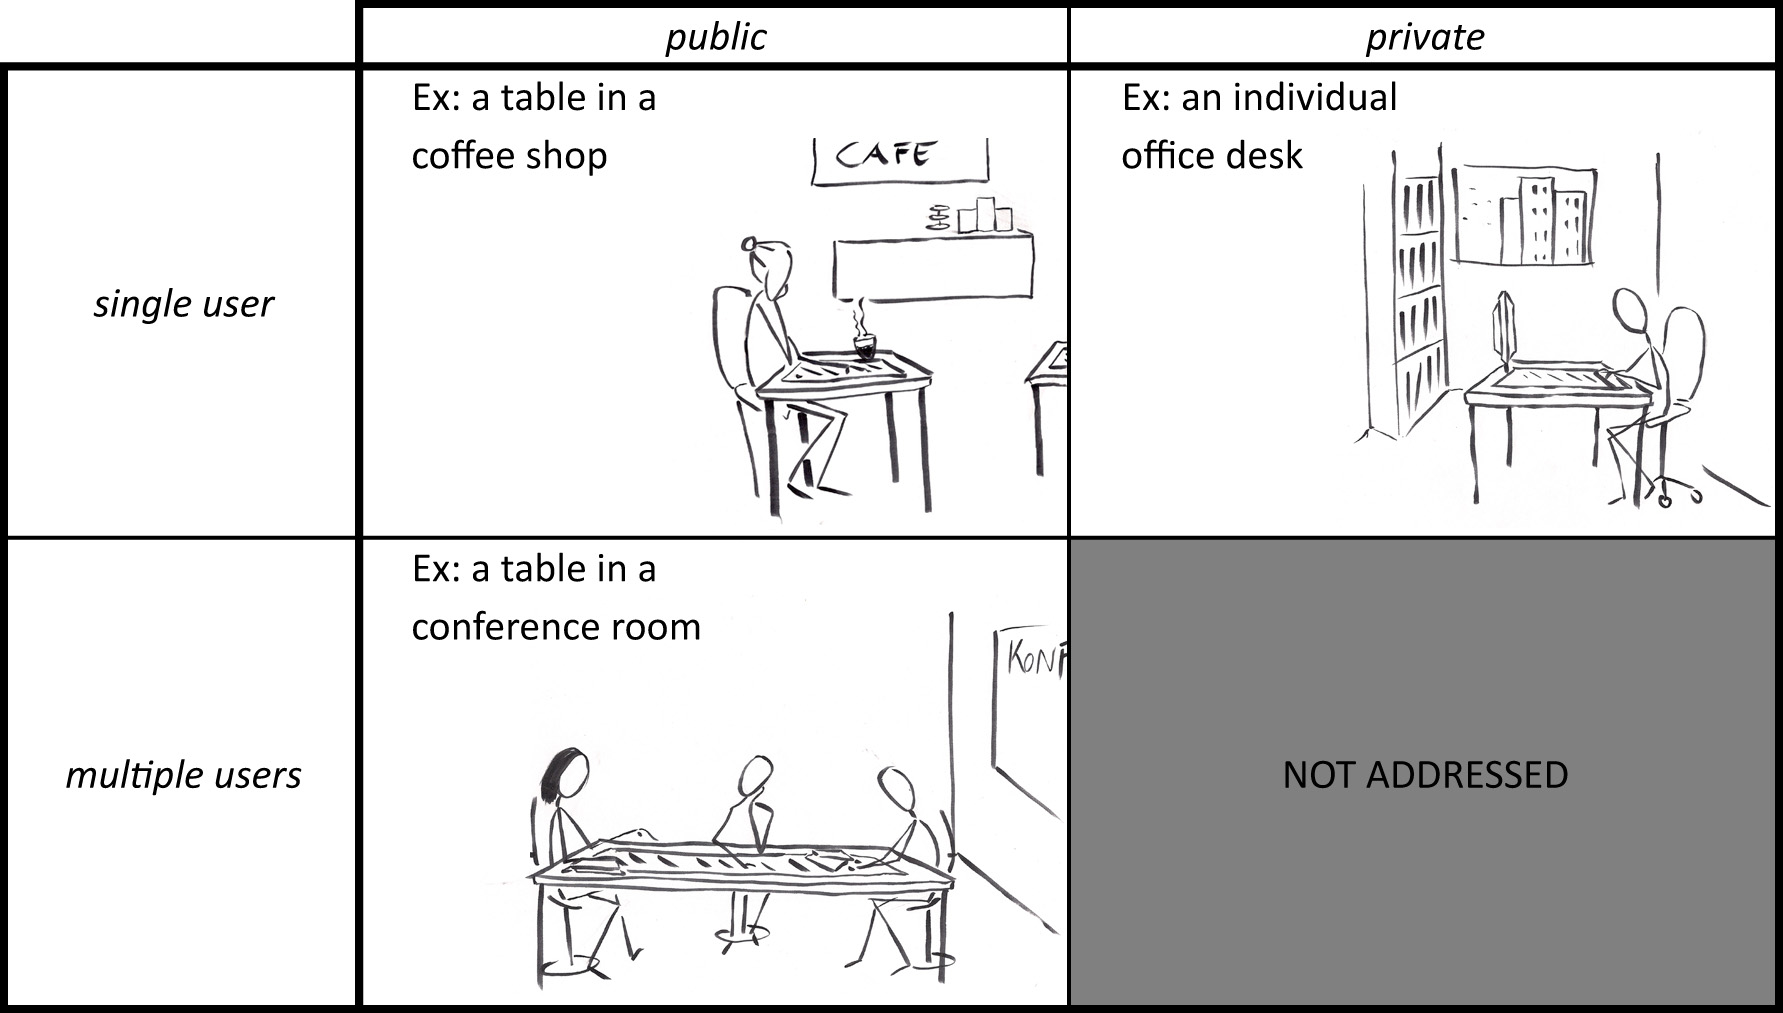
\includegraphics[width=0.8\textwidth]{images/marietable}
    \caption{The different situations in which the system can be used.}
    \label{fig:scenarios}
\end{figure}

Based on the level of privacy of the location (public/private) and the amount of involved users (single/multiple), four situations were identified.

However, the combination of multiple users in a private location was not addressed, for the reason that no design challenges specific to it were identified.
The challenges related to the multiple users were addressed by the situation \emph{multiple users with a public tabletop}; and the challenges related to the private aspect were addressed by the situation \emph{single user with a private tabletop}. 

The addressed situations are shown in figure~\ref{fig:scenarios}.

\subsubsection{Single user with a public tabletop}

This situation was derived from a scenario involving a person sitting alone at an interactive table in a coffee shop.

In this environment, the motivation for using the system is an activity that involves graphically intense content, such as 
internet browsing, reading, consulting a map, etc.
To start using the system, the user pairs the smartphone with the tabletop.
The process is quick and easy, but not completely automatic.
The user must explicitly allow the connection to be established.
The user does not usually need cables to use the smartphone.
Ideally, the connection with the tabletop is handled wirelessly.
The replicated UI appears on the tabletop, and the user starts interacting with the application.
The surface UI provides the user with features to manipulate the replicated UI, in particular: dragging, rotating and resizing.
Via the surface UI, the user can minimize and hide the replicated UI, as well as exit the application.

The smartphone itself is involved in the interaction.
Placing it on the table triggers the pairing process.
During the interaction, the replicated UI is collocated with the device, and moves together with it.
Lifting the smartphone off the table ends the connection.

%It should be possible for the user to wirelessly pair his/her personal device with a public tabletop computer.
%This implies that the devices are both connected to the local wireless networks, that they are able to detect each other and discover each other's identity on the network.
%It would not be safe to establish this connection automatically in a public space.
%Therefore, dialogs should be used both on the mobile device and on the tabletop to gather user input.
%The UI of the mobile device should be transferred to the interactive surface as graphical output, and this transferred display should be able to accept touch input to be forwarded back to the device.
%The transferred display should be contained in an application window, and this window should be manipulable (drag, resize, rotate, minimize, hide, ..).

%The application window should react to the state of the interactive surface.
%An example of this is that the application window should turn inactive if it is obstructed by an object on the table.

%\begin{itemize}
%\item{the mobile device is automatically detected by the tabletop}
%\item{dialog windows are displayed on both devices}
%\item{the wireless connection is automatic}
%\item{the mobile device UI is transferred to the surface.}
%\item{the transferred UI can be resized, rotated and moved on the surface}
%\item{the transferred UI goes inactive when objects obstruct it}
%\item{user input is forwarded to the mobile device}
%\item{the transferred UI can be minimized and restored}
%\item{the application can be exited by lifting the mobile device off the table.}
%\end{itemize}

\subsubsection{Multiple users with a public tabletop}

This situation was derived from a scenario involving some work colleagues having a meeting in a conference room, equipped with an interactive tabletop.
It can be argumented that such an environment is only partly public, being only accessible to the people working in the company.
However, in an effort to produce a design as generic as possible, and for the sake of simplicity, the tabletop is here considered a public device.

The motivation to use the system in this context is to view, comment and possibly edit digital data in a collaborative meeting.

Multiple users might want to connect their smartphones to the system simultaneously.
%This implies that the implementation should support parallel connections and simultaneous use.
Due to the lack of space on the table, the users remove their devices, but keep the replicated UI active on the tabletop.

%Mobile computing devices come in many forms, and ideally the system should support all of them.
%Devices vary in terms of software and hardware specifications.
%Some parameters that are especially important here are the programming platform, as well as the display resolution.

\subsubsection{Single user with a private tabletop}

This situation was derived from a scenario involving a user whose office desk is a tabletop.

The motivation for using the system is that it is a tool that the user interacts with daily, to support various activities related to the work routine.

The tabletop being private, can be configured to provide extended functionalities.
Examples of extended functionalities are; the pairing procedure can be made automatic and data can be shared between the devices.

%Some suggested functionalities are:
%\begin{itemize}
%\item automatic launch of the display extension application
%\item push application widgets from the extended display to the tabletop
%\item share data between the personal device and the tabletop
%\end{itemize}

\section{Solution requirements}
\label{sec:requirements}

Based on the analysis of the application context, the following requirements were derived.
Only the requirements that were relevant to the problem at hand were included.
They are divided into four categories, that each correspond to a different aspect of the system; the pairing procedure, the object tracking, the UI replication, and the surface UI.
\hfill\\
\hfill\\
The following fundamental requirement is not attached to any category, as it relates to several system aspects:
\begin{enumerate}[{R}-1]
\item \emph{The system should support multiple simultaneous devices.}
\end{enumerate}

\subsection{Pairing}

The pairing procedure is responsible for device discovery and connection.
It should fulfill the following requirements:

\label{RA}
\begin{enumerate}[{RA}-1]
\item Pairing the devices should be easy and quick.
\item Discovery between the devices should be automatic.
\item Establishing the connection should require explicit confirmation from the user.
%\item Automatic pairing should be an available option in trusted setups.
\item Closing the application should be easy and quick.
\end{enumerate}

%Connecting a personal device to a tabletop should be a quick and easy process.
%The system should include a detection mechanism that would allow the devices to become aware of each other, as well as a discovery protocol to gather the information necessary to the pairing, such as a Network IP.
%The connection should be wireless to guarantee a smooth experience.
%However, a public tabletop should not be allowed to gather data from, let alone connect to, a personal device without the explicit consent of its owner.
%In the case of a trusted setup, it should be possible to bypass any explicit user input.
%Exiting the application and closing the connection should also be easy, allowing the system to handle short successive sessions.

\subsection{Tracking}

Tracking the location of the smartphone on the tabletop allows to link specific features to the physical device.
It should fulfill the following requirements:

\label{RB}
\begin{enumerate}[{RB}-1]
\item Placing the smartphone on the tabletop should trigger the pairing procedure.
\item The replicated UI should be collocated with the smartphone, i.e.\ the replicated UI should be seemingly linked to the device, and should move when the device is moved.
\item Lifting the smartphone off the table should trigger the application exit.
\item It should be possible to remove the smartphone, but keep the replicated UI active on the tabletop.
\end{enumerate}

%It is a natural thing to place an object on a table, and tabletops are designed to allow for the integration of physical artifacts.
%Therefore, it should be possible to use the personal device as a tangible UI.
%For example, it would seem obvious that placing the device on the tabletop would launch the pairing process, or that lifting it off would interrupt the connection.
%Furthermore, it should be possible to control the position of the display extension by sliding the personal device on the surface.

\subsection{Replicated UI}

The replicated UI is the interactive mirror image of the smartphone displayed on the tabletop.
It should fulfill the following requirements:

\label{RC}
\begin{enumerate}[{RC}-1]
\item The UI of the smartphone should be replicated on the tabletop.
\item The graphical output from the smartphone should be dynamically relayed to the replicated UI.
\item The touch-based input from the replicated UI should be dynamically relayed to the smartphone.
\item The responsiveness of the replicated UI should be under 1 second, for the user experience to be satisfactory.
\end{enumerate}

%At the core of the system is the display extension.
%The UI of the personal device should be transferred to the tabletop, allowing the user to interact with it in a natural way.
%Graphical output from the personal device should be forwarded to the tabletop, and touch-based input from the tabletop should be forwarded to the personal device.

\subsection{Surface UI}

The surface UI is the interface on the tabletop that controls the replicated UI.
It should fulfill the following requirements:

\label{RD}
\begin{enumerate}[{RD}-1]
\item The surface UI should be easy to use.
\item The surface UI should allow the user to manipulate the replicated UI, i.e.\ the user should be able to move, rotate and resize the replicated UI across the tabletop display.
\item The surface UI should allow the user to minimize and restore the replicated UI.
\item The surface UI should allow the user to hide the replicated UI.
\item The surface UI should allow the user to close the replicated UI.
\item The surface UI should include controls that implement the functionalities provided by the physical buttons on the smartphone.
\end{enumerate}


%The user experience should be improved by using the display extension on the surface.
%Therefore, it is important to provide for a rich interaction.
%The transferred UI should be contained within a manipulable window on the tabletop.
%Specifically, the user should be able to move, rotate and resize the window; as well as minimize, hide and restore it.
%The system should include UI elements that implement the functions supported by the physical controls present on the personal device.
%Those elements and their function should be obvious to the user.
%
%%secondary features
%Modern smartphones include sensors that allow to switch the display orientation by tilting the device.
%This feature is strategic to certain applications, and should be implemented by the system.
%Obviously, tilting the tabletop is unfeasible, so another solution is necessary.
%
%As mentioned earlier, a tabletop's screen space would typically be shared among different applications and/or objects.
%Therefore, the system should handle limited screen space, and obstruction of the display extension.
%
%In a trusted setting, the user should have the possibility to push application widgets from the personal device to the tabletop, outside of the display extension, thus saving space on the latter.

\hfill\\
%As for the other system aspects, decisions were taken early in the process, that removed the need for a detailed design process.
It was agreed early in the process that three out of the four system aspects would not require a detailed design effort, for the following reasons.

First, it was decided that the pairing procedure should rely on already available solutions.
%as the focus of the thesis is not to contribute within this particular field.

Second, given that UI replication had already been decided upon, no design effort would be required for this system component.
%VNC was chosen as a protocol for UI replication, due to its stability and availability on most platforms.

Third, tracking the location of the smartphone is a technical requirement that does not require interaction design. %would only be used to trigger the pairing procedure.
\hfill\\
\hfill\\
The surface UI is the system component which supports the main user interaction.
As such, it poses the main design challenge, addressed hereunder in section~\ref{sec:interaction}.

\section{Designing the user interaction}
\label{sec:interaction}

This section focuses on the design of the surface UI, which comprises the UI elements that provide control over the replicated UI on the tabletop.

The input technique considered in the design of the surface UI is touch-based interaction.
The reason for this is that it is strongly consistent with the smartphone and tabletop experiences.
Both rely on touch-based interaction.
Moreover, the presence of other input peripherals cannot be expected, thus relying on touch-based input will ensure the system is usable in any setup.

The steps followed to design the surface UI were; (1) The generation of ideas (2) The definition of \emph{interaction strategies} (3) A study involving end-users to identify the interaction techniques that they find familiar.

%The pairing procedure does not introduce anything new to the field. There are known solutions to this challenge, which are described in section \ref{}.
%The remote UI replicates the UI of the personal device on the tabletop, and does not require any supplementary design.
%Using the personal device as a tangible UI for the display extension raises a series of design and implementation challenges. It is the opinion of the author that this research angle is promising, but it was decided to leave it out of the project for reasons of time constraints.
%\hfill\\

\subsection{Generating ideas}

The generation of ideas is an important part of the design process.
Benyon refers to it as envisionment \citep{Benyon:2010}, which he defines as the process of externalizing design thoughts.
The techniques that were used for this process are brainstorming, sketching, storyboarding and prototyping.

\subsubsection{Storyboards}

The scenarios included in appendix \ref{scenarios} were used as a base for the making of storyboards.
Storyboarding helped finding the general flow of the system interaction.
It also gave a visual dimension to the definition of the different system features, and raised new design issues.
%Putting orally expressed ideas on the paper is often a first test of their validity.

As an example, several system features were described in the initial scenarios as being the result of a tap on a button.
When storyboarding, it became obvious that having too many UI buttons would crowd the user interface.
This caused consideration of other interaction techniques, such as touch gestures.
Similarly, the issue of the location and size of the replicated UI on application launch first became apparent on a storyboard.

\subsubsection{Low fidelity prototypes}

Paper prototypes were used to aid the process of generating and evaluating as many design solutions as possible.
Screenshots of the iPhone UI \citep{iphone} were printed in various sizes, and used on a table to simulate interaction with the replicated UI.
Figure \ref{paperProt} shows some prototypes and a working session.

\begin{figure}[htb]
  \centering
    \includegraphics[width=1\textwidth]{images/paperProtDouble}
  \caption{Working with low fidelity prototypes.}
  \label{paperProt}
\end{figure}

%\begin{figure}[h!]
%  \caption{Low fidelity prototypes.}
%  \centering
%    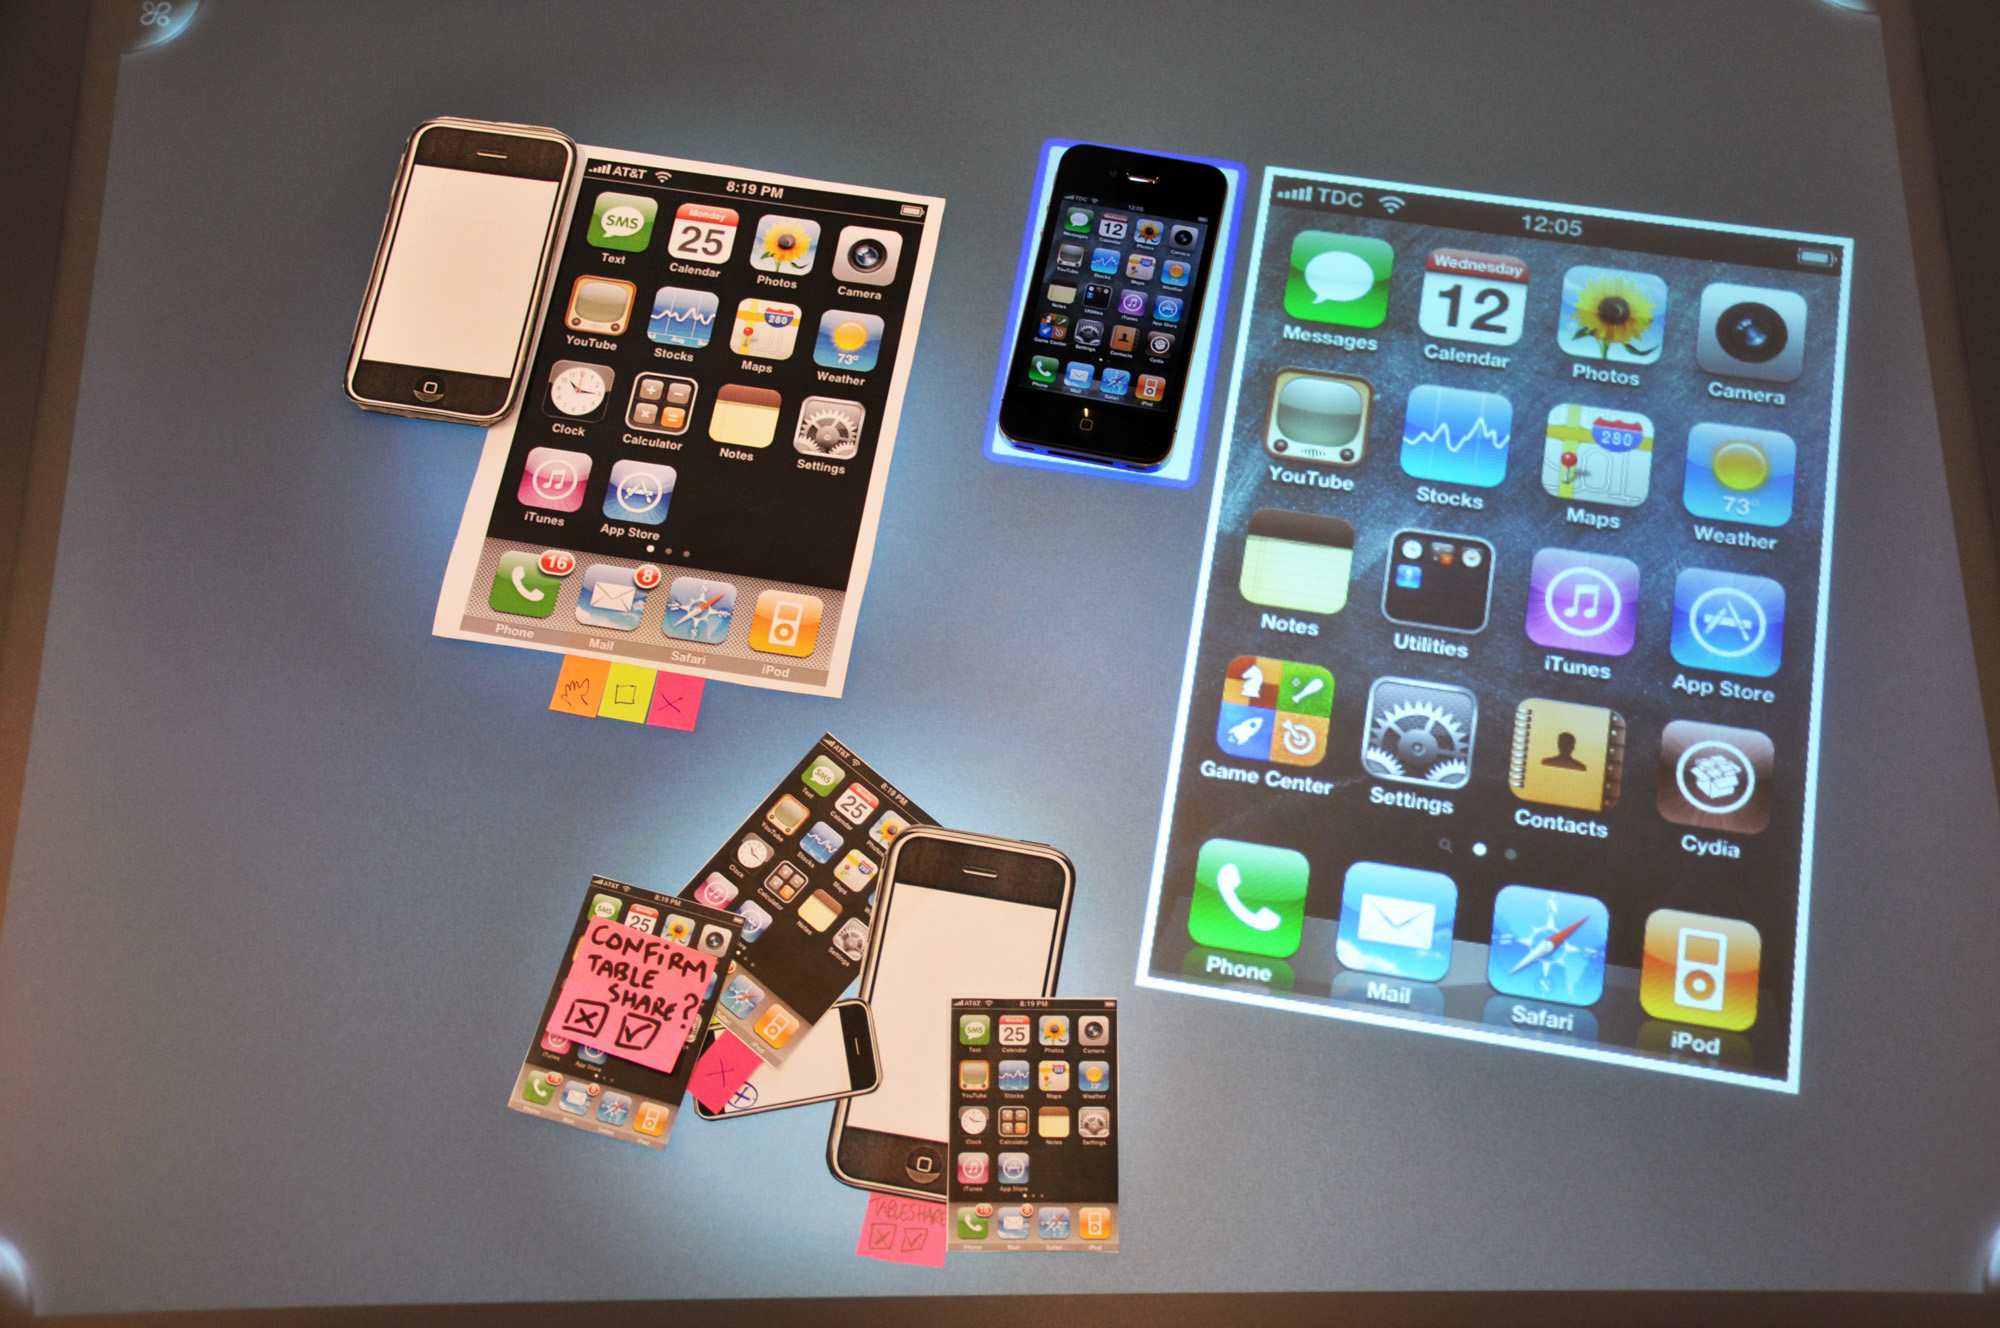
\includegraphics[width=0.8\textwidth]{images/paperprot2}
%\end{figure}

%\begin{figure}[h!]
%  \caption{Low fidelity prototypes.}
%  \centering
%    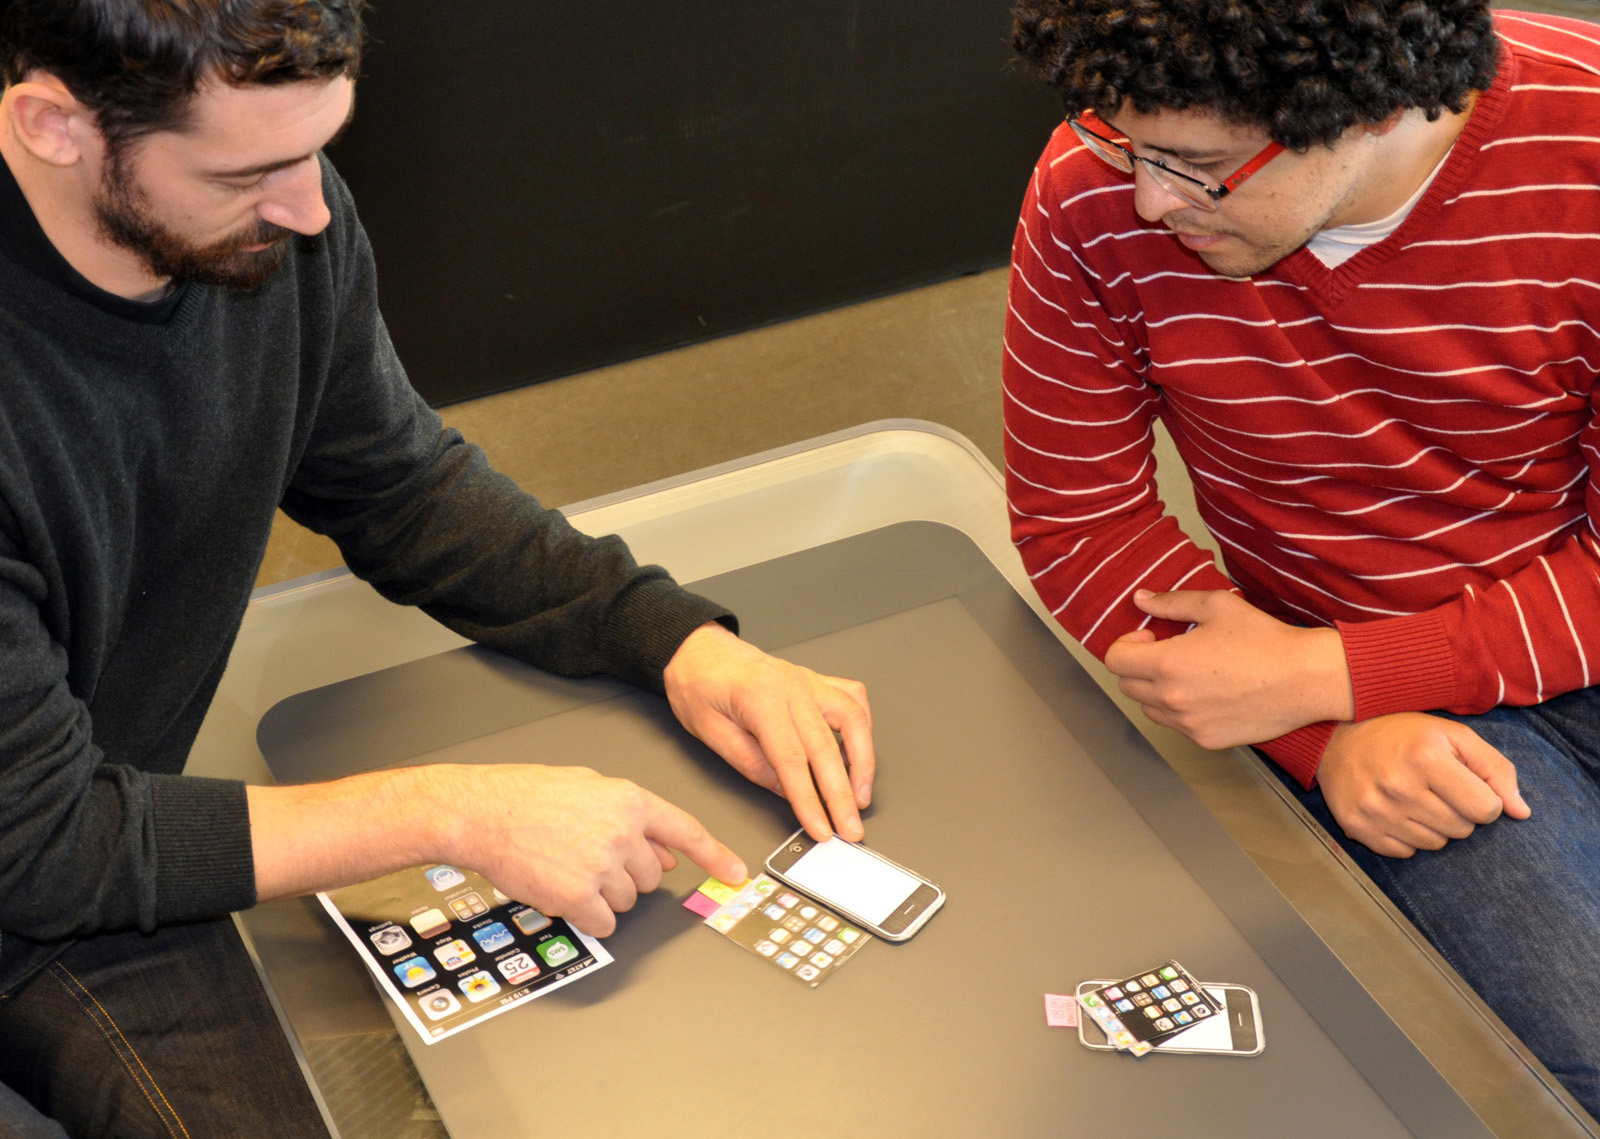
\includegraphics[width=0.8\textwidth]{images/paperprot3}
%\end{figure}

\subsection{Defining interaction strategies}
\label{sec:strategies}

The terms of \emph{actions} and \emph{commands} were used to refer to the different aspects of the user interaction.
They are inspired by the work done by Wobbrock et al. on defining hand gestures for interactive surfaces, \citep{Wobbrock:2009:gestures}.

A command is an \emph{effect} that the user wants to obtain, such as rotating a picture on a tabletop display.
An action is the \emph{cause} of an effect.
For example, using two fingers and performing a rotating gesture.
On a tabletop display, actions are typically hand gestures.

%Human computer interaction can be modeled as a simple cause-effect relationship.
%An action is a cause, a command is an effect, and together they form a single interaction between user and machine.

\subsubsection{Commands}

Based on the requirements formulated in section~\ref{sec:requirements} for the surface UI, the following six commands were identified.
They are the \emph{interaction primitives} for the surface UI, i.e.\ the commands that must be implemented by the surface UI, to allow the user full control of the replicated UI.

\begin{enumerate}
\item{\emph{Dragging} the replicated UI across the interactive surface.}
\item{\emph{Rotating} the replicated UI across the interactive surface.}
\item{\emph{Resizing} the replicated UI across the interactive surface.}
\item{\emph{Minimizing} the replicated UI, and restoring it.}
\item{\emph{Hiding} the content of the replicated UI.}
\item{\emph{Closing} the replicated UI.}
\end{enumerate}

Additionally, the surface UI should include controls that implement the functionalities provided by the physical buttons on the smartphone.

\subsubsection{Actions}

To invoke the commands that are defined above, a user needs to perform actions.
Various interaction techniques can be used to define these actions.
Figure~\ref{strategies} shows five \emph{interaction strategies} that were identified while working with paper prototypes.
Each strategy can be consistently implemented for all six interaction primitives.

\begin{figure}[htb]
\centering
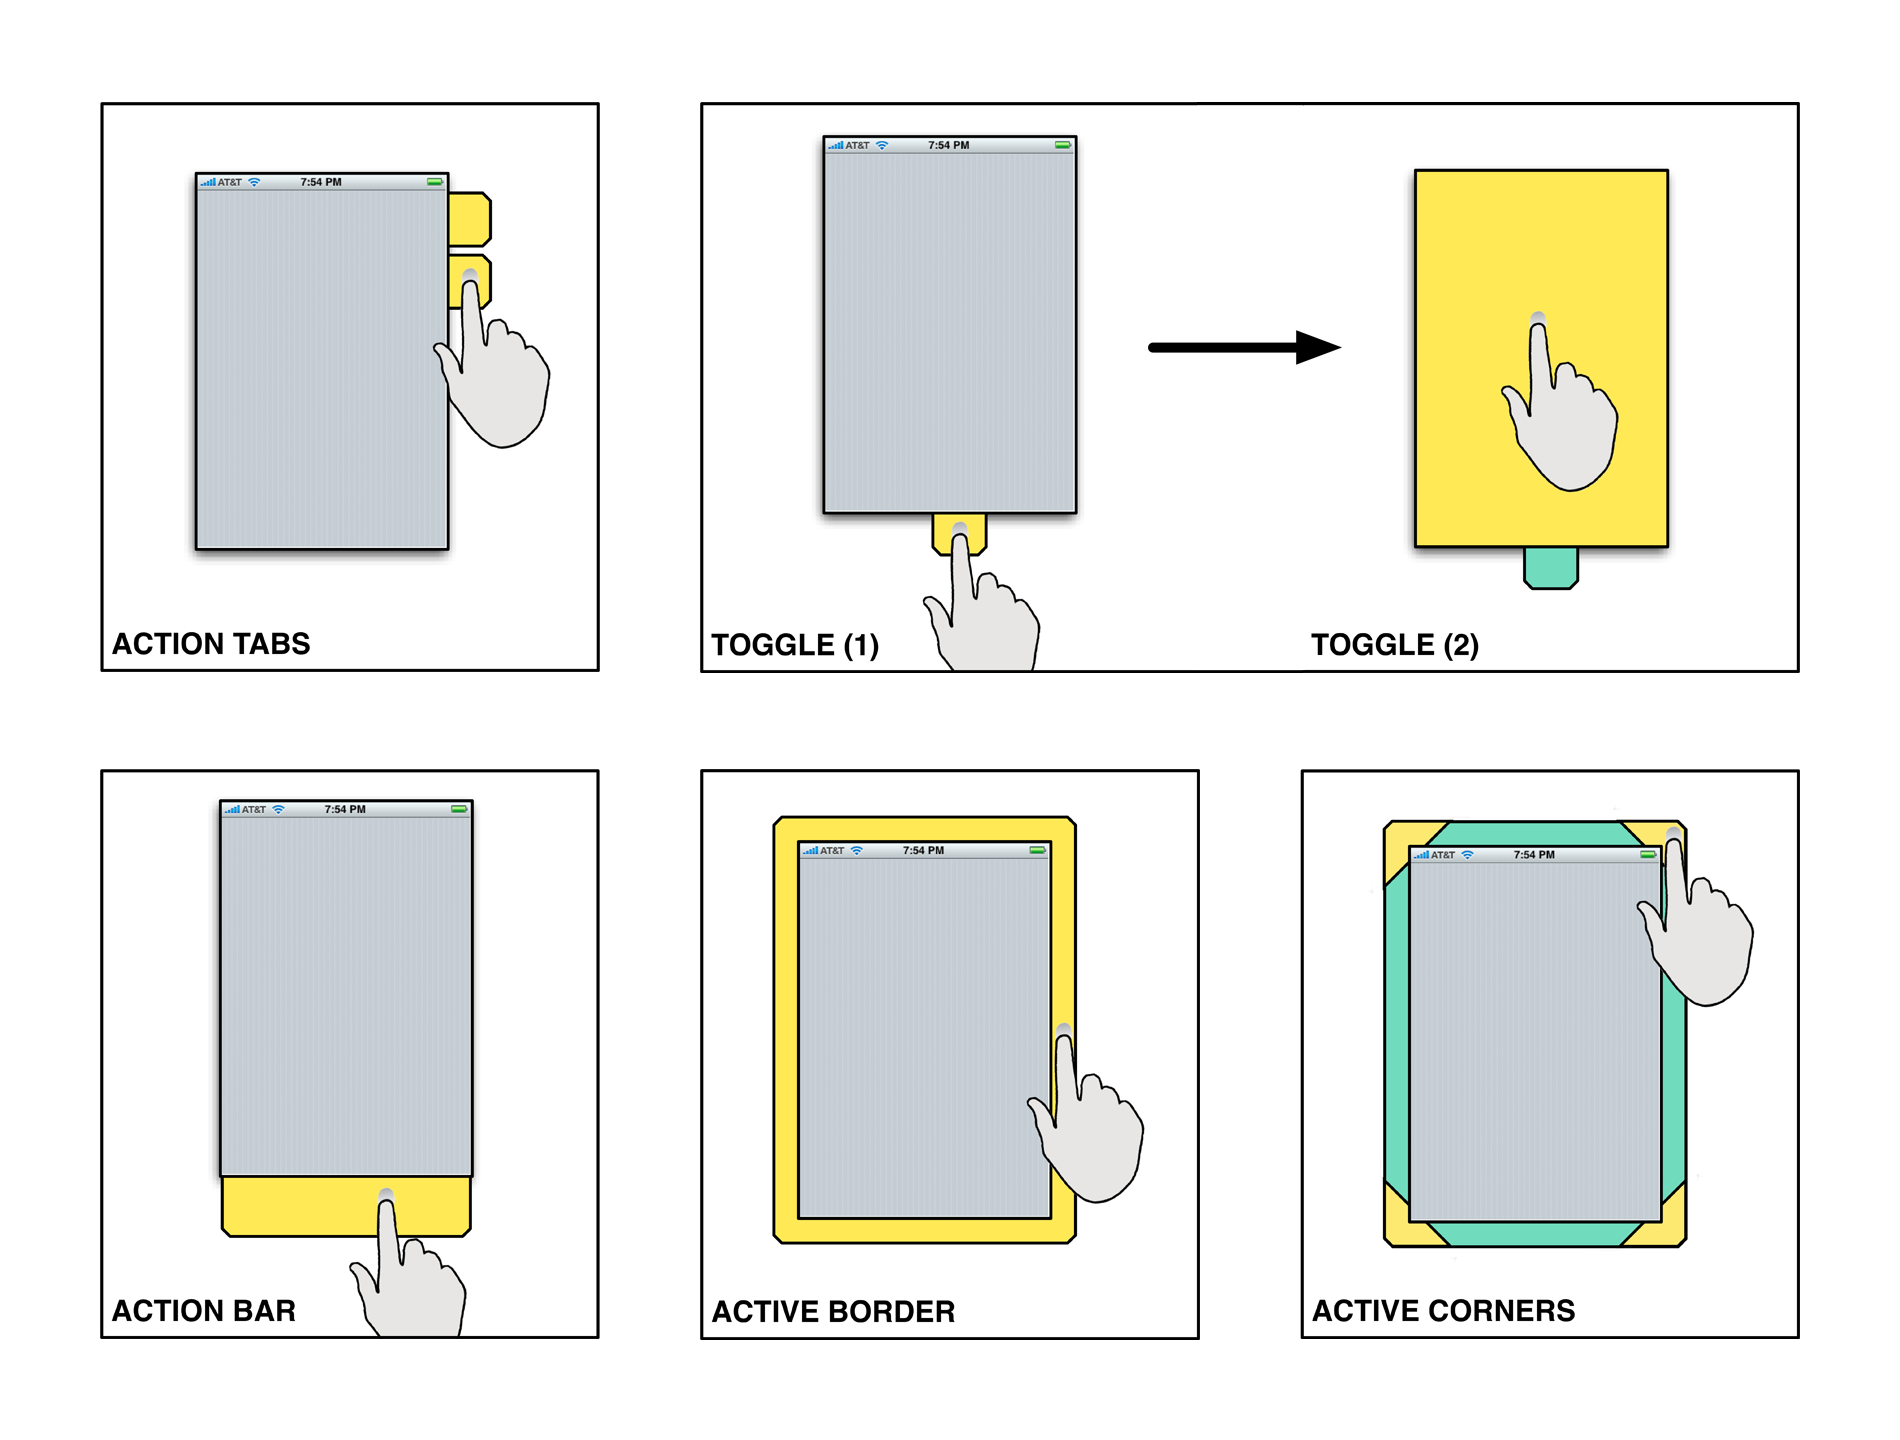
\includegraphics[width=1\linewidth]{images/strategies}
\caption{Interaction strategies.}
\label{strategies}
\end{figure}

\begin{enumerate}
\item{\emph{Action Tabs} are traditional buttons/tabs that implement functionalities.}
\item{\emph{Window Toggle} refers to using a switch to toggle the window between inactive and active states. In its inactive state, the window is made manipulable as a common digital picture.}
\item{The \emph{Action Bar} is a manipulation area which can be compared to a virtual touchpad.}
\item{The \emph{Active Border} is a digital frame around the application window used for manipulation.}
\item{\emph{Active Corners} is a strategy similar to Active Border, with the difference that the border's corners implement specific functionalities.}
\end{enumerate}

Beside these five interaction strategies, an additional category was used, that regrouped interaction techniques that did not correspond to any of the strategies.
This category is called \emph{Other}, and is explained on page~\pageref{other}.

%\begin{figure}[ht]
%\begin{minipage}[b]{0.5\linewidth}
%\centering
%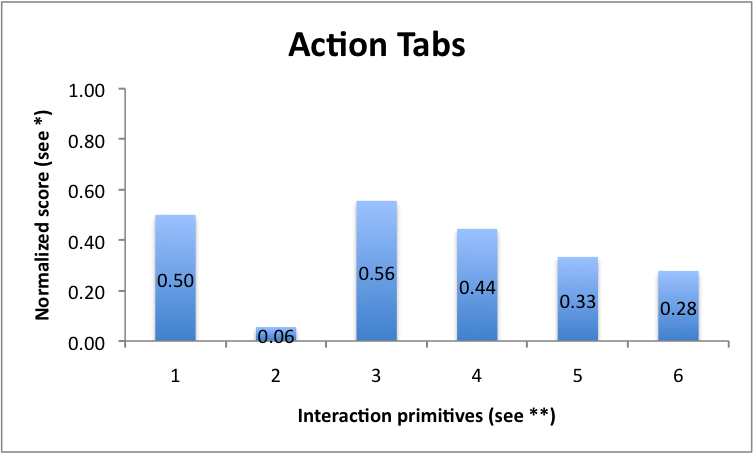
\includegraphics[width=0.6\linewidth]{images/strat1}
%\caption{action tabs prototype}
%\label{fig:strat1}
%\end{minipage}
%\hspace{0.5cm}
%\begin{minipage}[b]{0.5\linewidth}
%\centering
%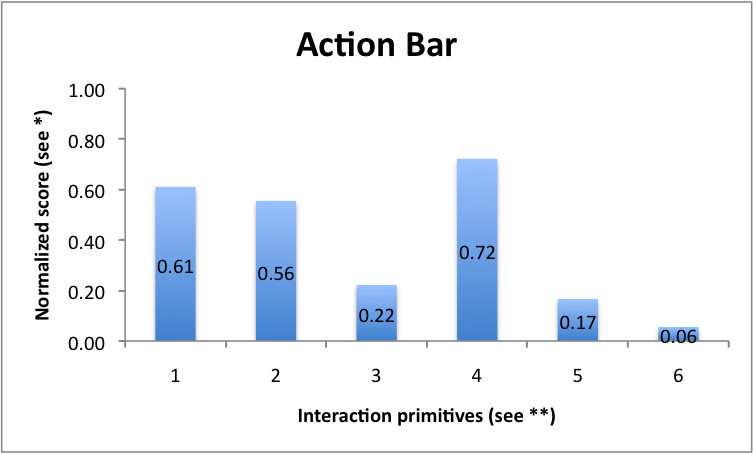
\includegraphics[width=0.6\linewidth]{images/strat2}
%\caption{action bar prototype}
%\label{fig:strat2}
%\end{minipage}
%\hfill\\
%\begin{minipage}[b]{0.5\linewidth}
%\centering
%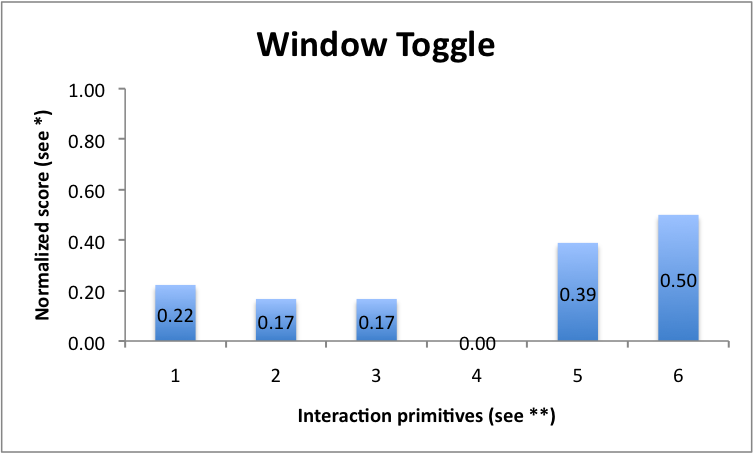
\includegraphics[width=0.6\linewidth]{images/strat3}
%\caption{active border prototype}
%\label{fig:strat3}
%\end{minipage}
%\hspace{0.5cm}
%\begin{minipage}[b]{0.5\linewidth}
%\centering
%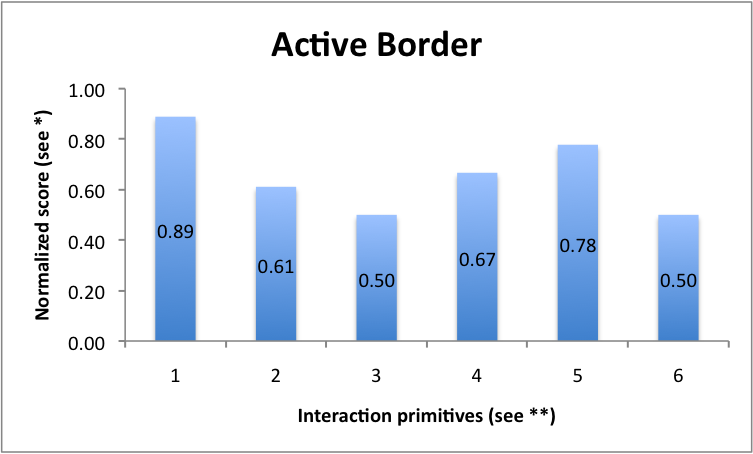
\includegraphics[width=0.6\linewidth]{images/strat4}
%\caption{active corners prototype}
%\label{fig:strat4}
%\end{minipage}
%\end{figure}

\subsection{Involving users}

To discover which of the defined interaction strategies were most intuitive, an experiment was carried out, that involved end users.
The experiment took the form of cooperative design sessions, where users engaged with low-fidelity prototypes of the system, in the aim of exploring and evaluating ideas.

The parameters of the experiment are the commands, also referred to as \emph{interaction primitives}, and the actions, also referred to as \emph{interaction strategies}, defined in section~\ref{sec:strategies}.

%The interaction primitives are central system features.
%For each primitive, the participants were asked to express an open-ended \emph{user suggestion}, then to \emph{rank} the interaction strategies.

\subsubsection{Experiment}

Twelve participants were recruited on a voluntary basis.
A session involved one participant and the designer, as shown in figure~\ref{fig:studyScreenshot}.
The participant sat next to the Microsoft Surface tabletop \citep{ms}, and was presented with an iPhone \citep{iphone}, but both devices were turned off.
On the tabletop were paper prototypes, that were to be used as representations of UI elements throughout the session.
The designer lead the experiment by reading instructions from a script (included in appendix~\ref{app:study}) and answering the participant's questions.

\begin{figure}[htb]
  \centering
    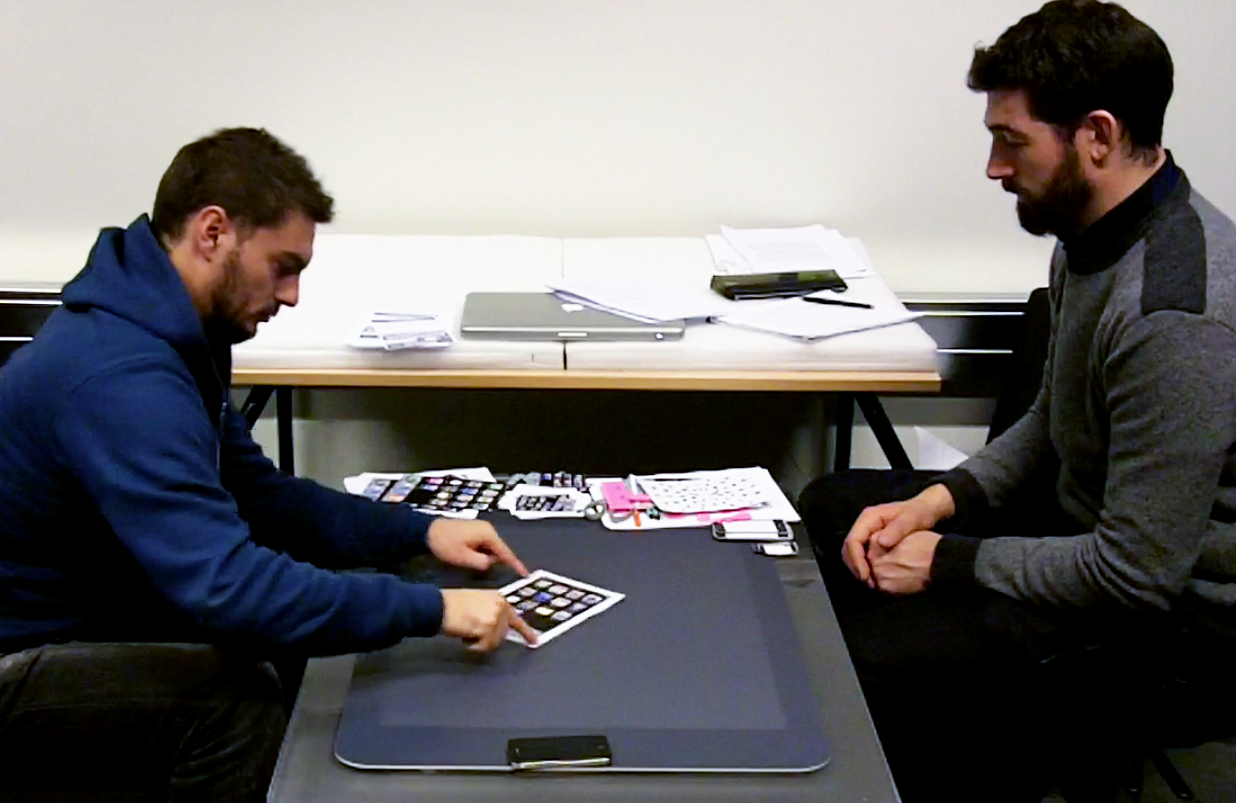
\includegraphics[width=0.7\textwidth]{images/studyScreenshot}
  \caption{Designing the surface UI with paper prototypes.}
  \label{fig:studyScreenshot}
\end{figure}

As an introduction, the following things were explained to the participant:
\begin{itemize}
\item The purpose of the experiment
\item The purpose of the application
\item The tasks that the participant will perform
\item The principles of working with paper prototypes
\end{itemize}
\hfill
\linebreak
The session revolved around a task that the participant was asked to perform using the prototyped application.
The task was to write an email, and it required the user to go through six phases.
Each phase was dedicated to an interaction primitive, and they had the same structure, which is as follows:
\begin{enumerate}
\item The primitive was explained to the participant in terms of a command to the application.
\item The user was asked to express an open-ended suggestion, i.e.\ suggest an action that s/he would perform to obtain the desired effect, and to demonstrate the action using the prototypes,
\item The designer described action suggestions, that the user was asked to try out and rank by order of preference.
\end{enumerate}

%There is a seventh phase focusing on the pairing procedure.
%This phase occurs first and is meant as an example to the participant, describing the common structure.
%At the end of this phase, a slide animation is used to describe all six primitives to the user.
\hfill\\
For each command, there is a total of six possible actions.
However, only half of the actions were presented to each participant, to avoid overwhelming them. 
%However, it was decided that presenting a user with six options to rank would be overwhelming.
%The volunteers were therefore split into two groups, each evaluating a subset of the interaction strategies.
%The repartition is shown in table~\ref{groups}.
%
%\begin{figure}[htb]
%  \centering
%    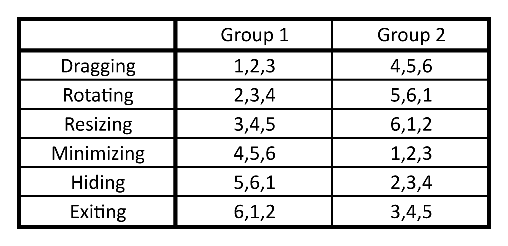
\includegraphics[scale=1]{images/groups}
%  \caption{The repartition of the evaluated interaction strategies between the two groups of participants. The strategies are 1)~Action Tabs 2)~Action Bar 3)~Window Toggle 4)~Active Border 5)~Active Corners 6)~Other.}
%  \label{groups}
%\end{figure}

\subsubsection{Data processing}

Participant answers were gathered in a form such as the one included in appendix~\ref{app:studyForm}.
The form is a matrix where an entry corresponds to a pair (primitive, strategy).
The entries contain the position from first (highest) to third (lowest), that was given by the user for using the suggested strategy for implementing the primitive.
After processing all answers, each entry contained six positions.
In order to obtain a numeric score for each entry, a weighted average was calculated.
A weight of 3 was given to a first position, a weight of 1 to a second position, and a weight of 0 to a third position.
Finally, the results were normalized to a [0-1] interval, where a 1 meant that the entry was awarded a first position by all participants, and a 0 meant that all participants ranked the entry third.
Figure~\ref{resultMatrix} summarizes the normalized scores, with colored cells containing values above 0.6.
This is considered a superior score, because it can only be obtained if half of the participants awarded the first position.
%The same results are presented in the form of charts in figure~\ref{primitives}.

The experiment data also included the user suggestions, gathered separately on paper.
User suggestions were not limited to one per primitive.
Thus, the processed data was a disparate list of suggestions that each had a counter variable indicating how many users independently expressed said suggestion.

\begin{figure}[htb]
  \centering
    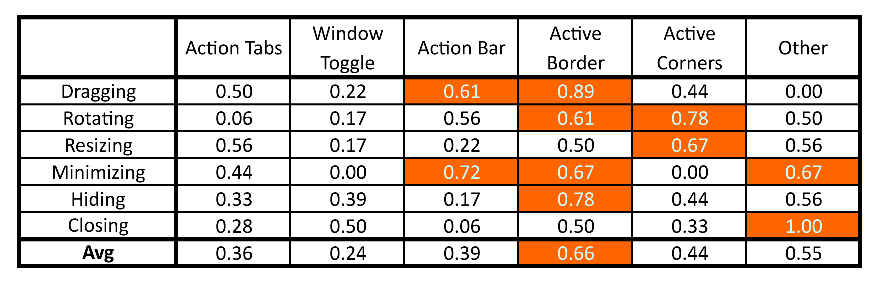
\includegraphics[scale=1]{images/resultMatrix}
  \caption{Normalized weighted average of the ranks given to each pair (primitive, strategy).}
  \label{resultMatrix}
\end{figure}

%\begin{figure}[h!]
%  \centering
%    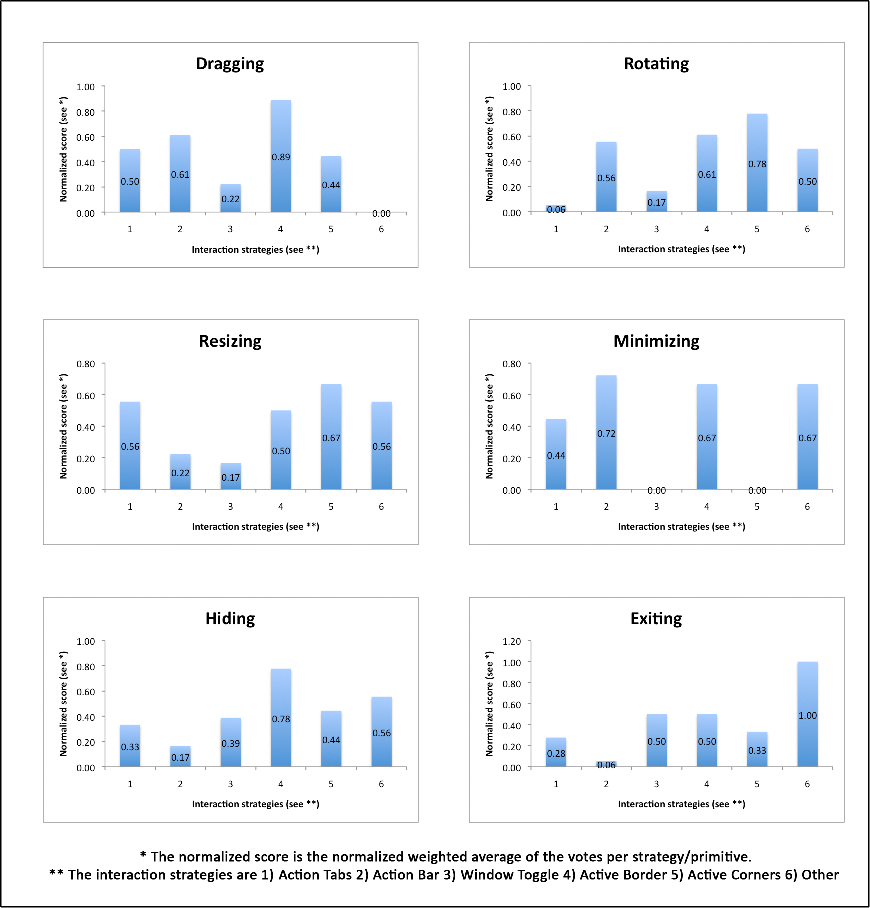
\includegraphics[width=1\textwidth]{images/primHistog}
%    \caption{The score of the different interaction strategies for each primitive.}
%	\label{primitives}    
%\end{figure}

\subsubsection{Result Analysis}

It is possible to divide the primitives into two groups.
The first half---dragging, rotating, resizing---have a concrete visual signification.
The second half---minimizing, hiding, closing---are more abstract.

For the first three primitives, there is a strong coherence in the choice of the participants.
The favored strategies are the active border, the action bar and active corners.
All three require the user to interact with an area directly around the window in order to manipulate it and modify its position, orientation or size.
This interaction technique is similar to the current standard for manipulating pictures on interactive screens.
However in the present case, the replicated UI is logically avoided because of its role as IO relay between the tabletop and the smartphone.

For the last three primitives, the action bar and active border continue to score high, even though there is no apparent relation between the visual aspect of the strategy and the effect implied by the command.
To understand this, it is necessary to look at the actual suggestions.
The favored strategies for minimizing were double tapping on the action bar and double tapping on the active border.
For hiding, the favored strategy was double tapping on the active border.
It is thus obvious that it is the double tap that participants have a preference for, possibly because it is a common technique in many other application contexts, as well as a quick and easy one.
\\
\linebreak
\label{other} It is not possible to analyze the scores of the sixth category as a whole, as it does not represent a consistent strategy, but more a patchwork of various suggestions. They are:
\begin{enumerate}
\item Drag by holding a finger on a specific tab, and using another finger to tap a destination target to move the window
\item Rotate by performing a one finger dragging gesture on a corner of the window
\item Resize by pulling the window apart with both hands
\item Minimize by dragging the window to the bottom of the surface
\item Hide by placing and holding a hand on the window
\item Close by dragging the window to a specific location on the surface
\end{enumerate}
Suggestions 4 and 6 are similar, and they are the only ones that scored above 0.6.
This suggests that moving the window off screen; is a natural way to remove focus from the application.
Interestingly, this correlates with the analysis of the user suggestions, presented hereunder.

\subsubsection{User suggestions}

The user suggestions were multiple and heterogeneous, but data processing revealed a clear tendency in three situations.

In the case of dragging, half of the participants suggested using one or more fingers to touch within the replicated UI, and perform a drag gesture.
This is interesting, because it is an obvious conflict for the developer, i.e.\ any touch inside the replicated UI is forwarded to the smartphone, and logically can not be interpreted by the surface UI.
It must be noted that dragging was the first primitive, and it can therefore be assumed that the participants did not yet have a full understanding of the application concept.
However, this result shows what the ideal system should be able to do, namely interpret the intention of the user.

In the case of resizing, 8 out of 12 participants suggested grabbing the sides of the window with two fingers, and pulling the window apart to enlarge it.
This shows that the gesture is very intuitive, and that implementing it would definitely add to the usability of the system.

The third consensus was for minimizing, where 7 out of 12 participants suggested dragging the window offscreen (or to a specific location along the surface edge).
The same suggestion reoccurred for the primitives hiding and closing, though with less decisiveness.
Once again, it shows that the gesture is an intuitive one.
Moreover, it is consistent with the action of removing a real piece of paper from the center of a table.
%, and the act of minimizing, hiding or closing the display extension application.
%Moving the application out of focus seems like a good solution, and using a simple dragging gesture is a natural way of doing it.

\clearpage
\section{Final design of TIDE}
\label{sec:design}

Based on the design analysis and in particular the feedback from the user experiment, the following design decisions were taken.
They relate to the requirements defined in section~\ref{sec:requirements}.
%In the continued effort to build an intuitive system, that provides a spontaneous user interaction, special focus was given to the design consistency, and in particular:
%\begin{itemize}
%\item The design should be consistent with itself. If the features are coherent, the user will be able to derive one from the other.
%\item The design should be consistent with the user background. In the present case, the user already has some expertise with a smartphone. Therefore, the design should be consistent with the touch-based interaction that is provided on most smartphones.
%\item The design should be consistent with the physicality of the devices. In particular, the tabletop form has implications on the user's expectations.
%\end{itemize}
\\
\linebreak
The requirement \emph{R-1 The system should support multiple simultaneous devices} will be fulfilled by the following design decision.
\begin{enumerate}[{D}-1]
\item The system will be implemented with focus on loose coupling between the main application session classes and the objects handling individual devices, in order to support simultaneous devices, as shown in figure~\ref{fig:sq2phones}. 
\end{enumerate}
\begin{figure}[htb]
  \centering
    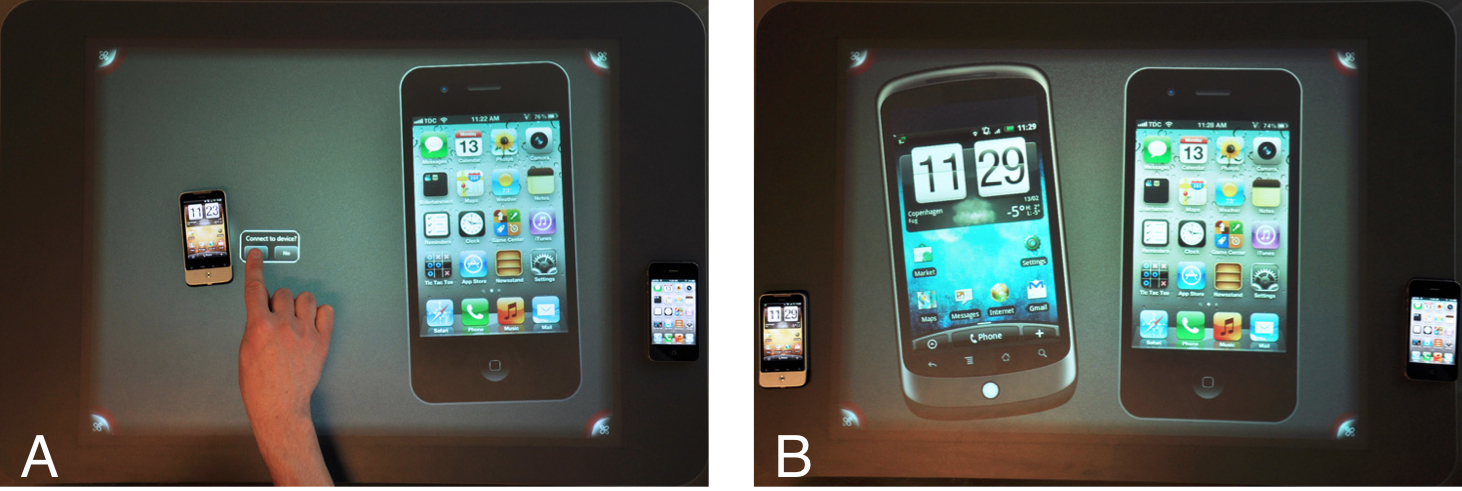
\includegraphics[width=0.7\linewidth]{images/sq2phones}
  \caption{(A) Pairing second device (B) Simultaneous devices}
  \label{fig:sq2phones}
\end{figure}

\subsection{Pairing}

The following design decisions address the requirements RA-1 to RA-4 (see p.~\pageref{RA}).

\begin{enumerate}[{DA}-1]
\item \hfill
	\begin{enumerate}[{DA-1}a]
	\item Pairing is triggered by placing the smartphone on the tabletop, as shown in figure~\ref{fig:sqPair}, for the reason that it is a simple gesture that is consistent with the form of the tabletop.

\begin{figure}[htb]
  \centering
    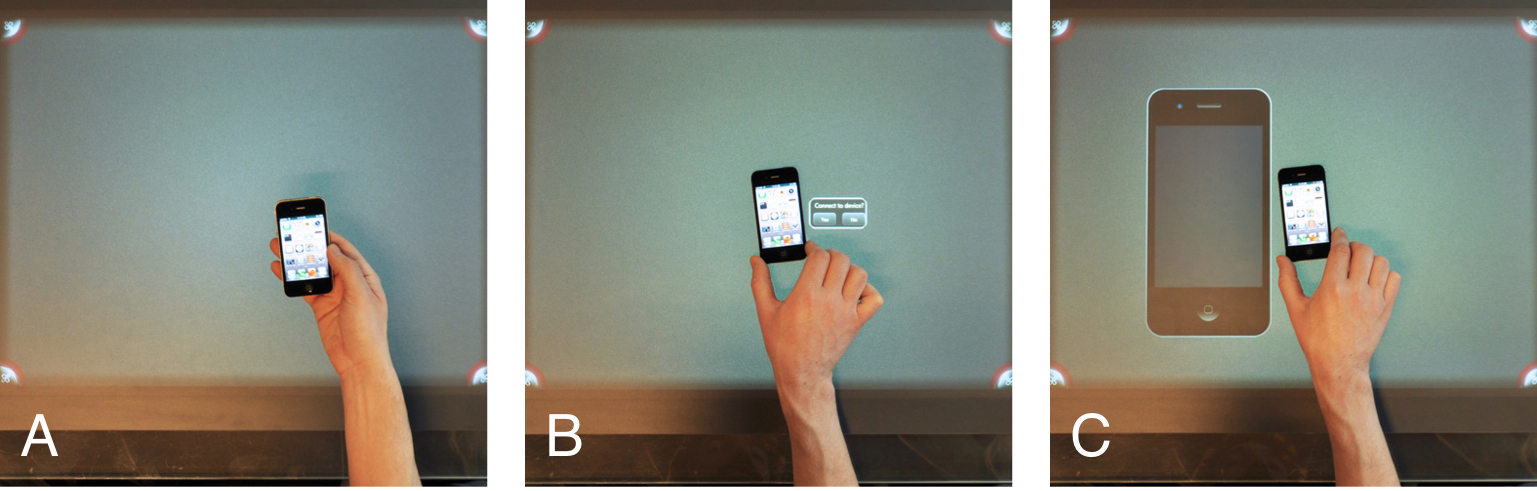
\includegraphics[width=0.7\linewidth]{images/sqPair}
  \caption{(A) Device in hand (B) Device detected (C) Device connected}
  \label{fig:sqPair}
\end{figure}

	\item Pairing is based on wireless connectivity, in order to provide spontaneity to the interaction.
	\end{enumerate}
\item Device discovery relies on a standard networking protocol, in order to make it automatic, and provide spontaneity to the interaction.
\item The user must confirm the connection, both on the tabletop and on the smartphone, for reasons of security.
The tabletop should not be allowed to connect to an unknown device without explicit authorization, but the user should also be able to confirm that the smartphone is the correct one.
\item See DD-5.
\end{enumerate}

\subsection{Tracking}

The following design decisions address the requirements RB-1 to RB-4 (see p.~\pageref{RB}).

\label{DB}
\begin{enumerate}[{DB}-1]
\item Smartphones that come in contact with the tabletop are detected, using computer vision and shape recognition.
\item The locations of the smartphones on the tabletop are tracked, using computer vision.
\item Removal of smartphones are detected using computer vision.
\item The replicated UI can be made active on the tabletop independently of the smartphone.
\end{enumerate}

\subsection{Replicated UI}

The following design decisions address the requirements RC-1 to RC-4 (see p.~\pageref{RC}).

\begin{enumerate}[{DC}-1]
\item The smartphone screen is replicated to the tabletop, using a standard desktop sharing protocol, for the reason that such protocols are platform independent and stable.
\item See DC-1.
\item See DC-1.
\item See DC-1.
\end{enumerate}

\subsection{Surface UI}

The following design decisions address the requirements RD-1 to RD-6 (see p.~\pageref{RD}).
It was decided to use multiple techniques to activate certain features.
The reason for this is to benefit from the advantages of all interaction techniques.
Some are easy to discover, and provide the learnability and intuitiveness that is looked for, while others are quicker and easier to use.
This is standard practice within software design, a good example being keyboard shortcuts, that are not easily discovered by a novice user, but are preferred by the expert user for their efficiency.

\clearpage

\label{DD}
\begin{enumerate}[{DD}-1]
\item The surface UI takes the form of an active border that contains the replicated UI, based on the user feedback.
It is a virtual replication of the physical body of the smartphone, to provide consistency in the user experience.
\item The replicated UI can be manipulated by using touch-based gestures on the surface UI, for reasons of consistency with both the smartphone and tabletop experiences.
	\begin{enumerate}[{DD-2}a]
	\item Dragging is done by performing a dragging gesture with one or more fingers.
	\item Rotating is done by
		\begin{enumerate}[1{.}]
		\item Dragging the corner of the surface UI, as shown in figure~\ref{fig:sq1f}

\begin{figure}[htb]
  \centering
    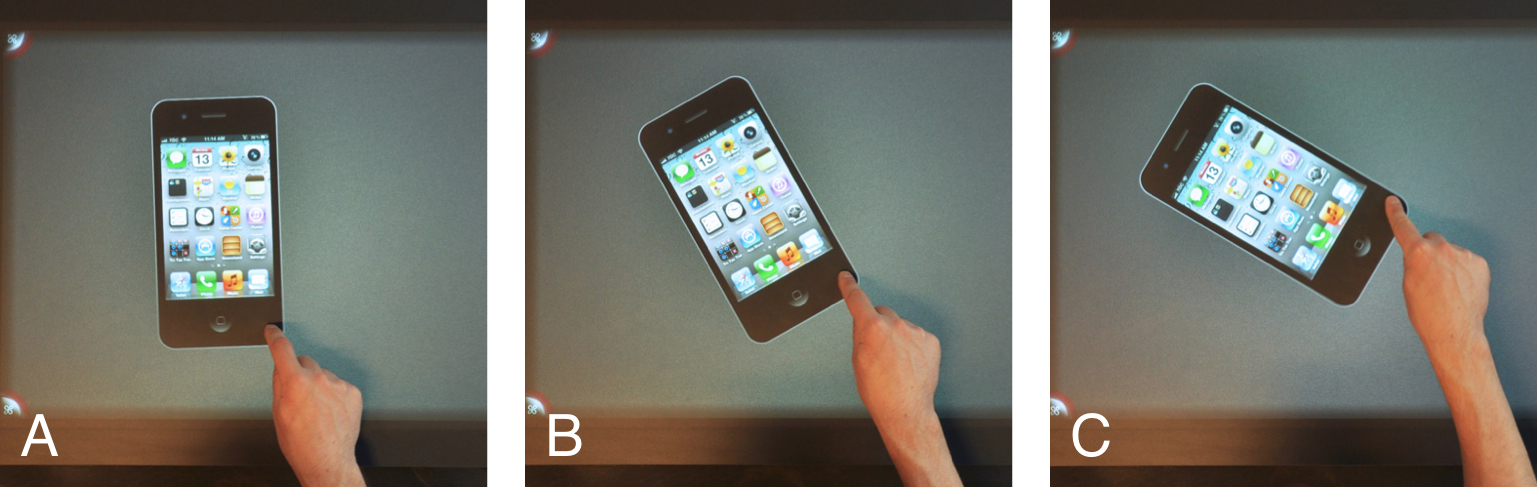
\includegraphics[width=0.7\linewidth]{images/sq1f}
  \caption{(A,B,C) Rotating using 1 finger.}
  \label{fig:sq1f}
\end{figure}

		\item Performing a rotating gesture with two fingers of the same hand, as shown in figure~\ref{fig:sq2f1h}

\begin{figure}[htb]
  \centering
    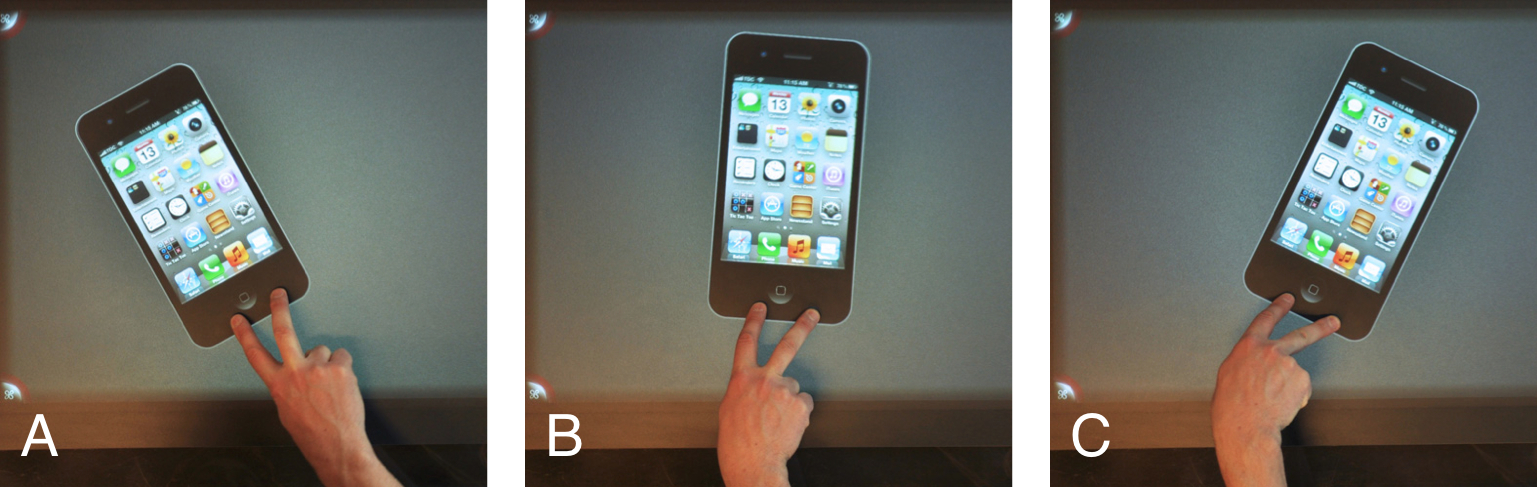
\includegraphics[width=0.7\linewidth]{images/sq2f1h}
  \caption{(A,B,C) Rotating using 2 fingers of the same hand.}
  \label{fig:sq2f1h}
\end{figure}

		\item Performing a rotating gesture with two hands
		\end{enumerate}
\clearpage


	\item Resizing is done by
		\begin{enumerate}[1{.}]
		\item Performing a pinching gesture with two fingers of the same hand
		\item Performing a resizing gesture with two hands, as shown in figure~\ref{fig:sqResize}
		
\begin{figure}[h!]
  \centering
    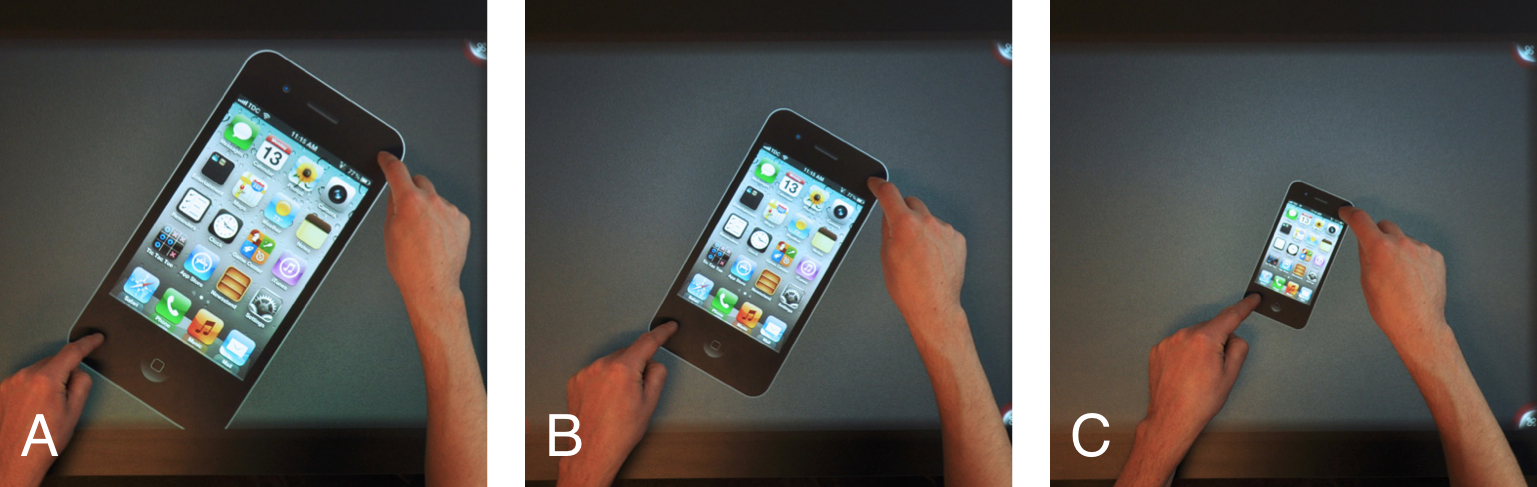
\includegraphics[width=0.7\linewidth]{images/sqResize}
  \caption{(A,B,C) Resizing down using both hands.}
  \label{fig:sqResize}
\end{figure}
		
		\end{enumerate}
	\end{enumerate}
\item Minimizing the replicated UI can be done by
	\begin{enumerate}[1{.}]
	\item Resizing the surface UI down
	\item Dragging the surface UI off an edge of the table, as shown in figure~\ref{fig:sqMin2}

\begin{figure}[htb]
  \centering
    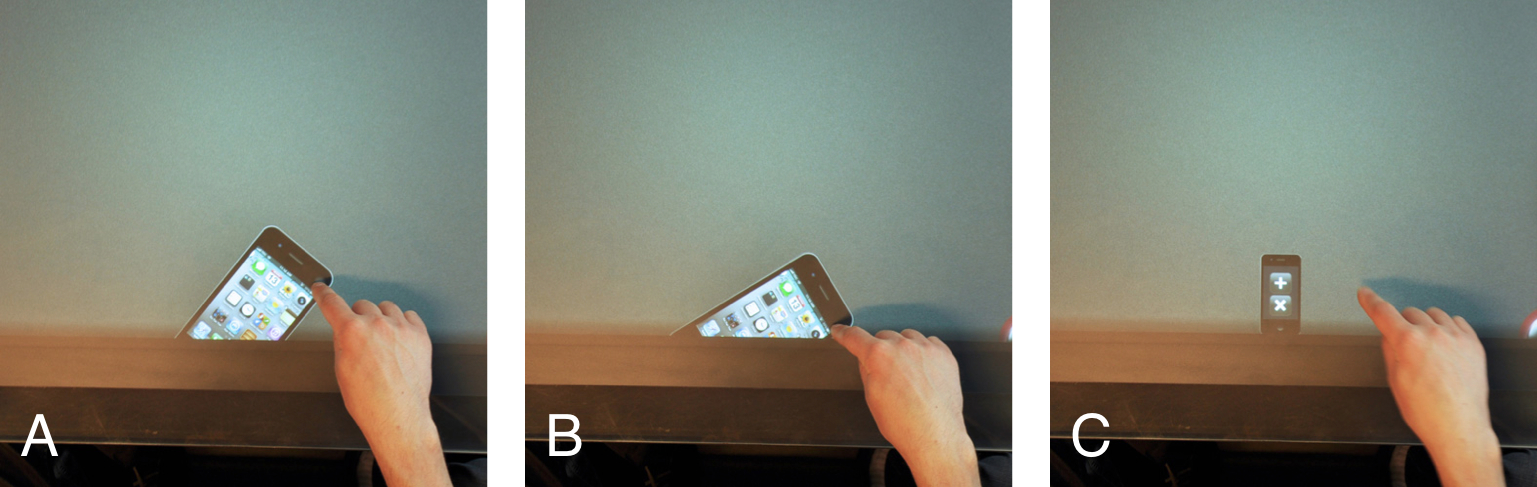
\includegraphics[width=0.7\linewidth]{images/sqMin2}
  \caption{(A,B,C) Minimizing by dragging off the edge.}
  \label{fig:sqMin2}
\end{figure}
	
	\item Double tapping the surface UI, as shown in figure~\ref{fig:sqMin1}
	\item Placing a full hand on the surface UI, as shown in figure~\ref{fig:sqMin1}
	\end{enumerate}
	
\begin{figure}[htb]
  \centering
    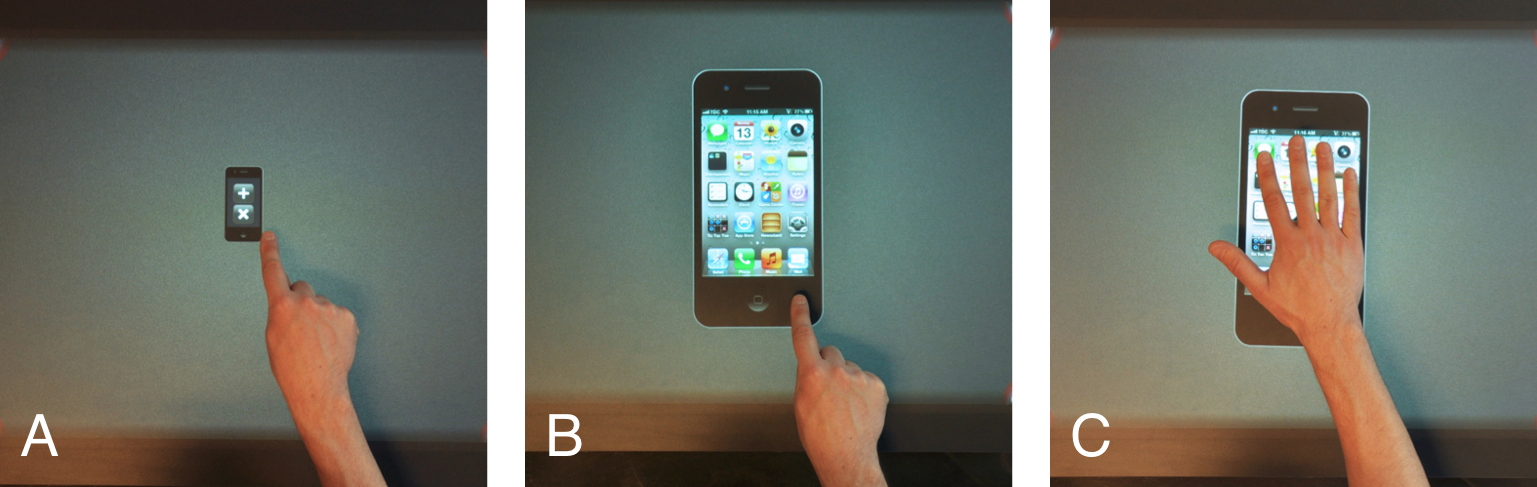
\includegraphics[width=0.7\linewidth]{images/sqMin1}
  \caption{(A) Minimized state (B) Double tap (C) Whole hand tap}
  \label{fig:sqMin1}
\end{figure}

When minimized, the surface UI appears as an icon on the tabletop, and can be restored by tapping a button.
\item Hiding the replicated UI is done by minimizing the surface UI, based on user feedback, see DD-3.
\item Closing the replicated UI is shown in figure~\ref{fig:sqClose}, it can be done by
	\begin{enumerate}[1{.}]
	\item Closing the minimized surface UI
	\item Dragging the surface UI to a corner of the tabletop
	\item Pressing and holding a finger on the active border
	\end{enumerate}

\begin{figure}[htb]
  \centering
    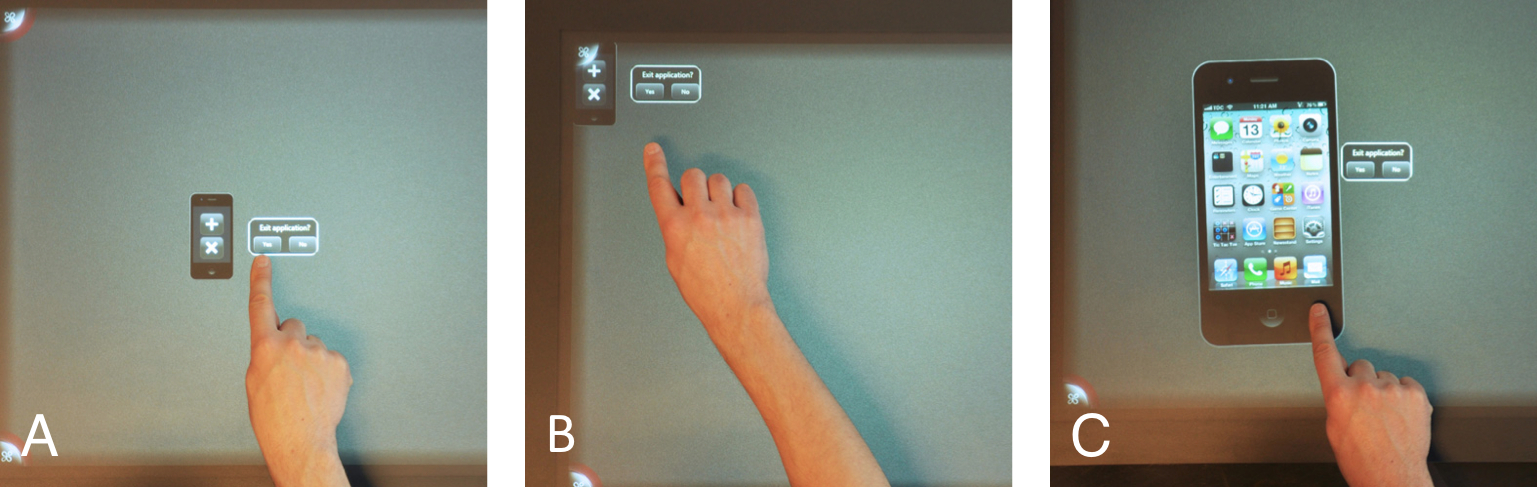
\includegraphics[width=0.7\linewidth]{images/sqClose}
  \caption{(A) Minimize then close (B) Close by dragging to a corner (C) Press and hold to close}
  \label{fig:sqClose}
\end{figure}

\item The functionalities provided by the smartphone's physical buttons can be accessed by tapping virtual replications of the buttons on the surface UI.
\end{enumerate}

\firmlists




%%%%%%%%%%%%%%%%%%%%%%
%%% IMPLEMENTATION %%%
%%%%%%%%%%%%%%%%%%%%%%

\chapter{The TIDE application: Tabletop Interactive Display Extension for mobile devices}
\label{system}

refer to problem formulation:

Following is an open list of problems that we will address in order to achieve device composition by means of implicit interaction.
\begin{enumerate}
\item{\emph{Setup}: How is a device enabled for integrating with a tabletop?
The setup should be simple, to be performed only once by non-technical users.
An initial survey of possible solutions points towards the use of tagging mechanisms and/or camera-based object recognition.}
\item{\emph{Discovery}: How do the tabletop and the device discover and communicate with each other?
How do we solve the issues of discovery, handshake, network connectivity, and encryption mechanisms to ensure privacy?}
\item{\emph{UI transfer}: Given the computational constraints of mobile devices, how can the UI transfer be efficiently implemented so as to support native applications and guarantee a seamless user experience?}
\item{\emph{Input}: How can the users interact with their applications on the tabletop (touch and other peripherals)?}
\item{\emph{Interaction Design}: What means of interaction are best-fitted for the tabletop-based systems that we propose to develop?
How can we best adapt to public/private uses and single/multiple users?
How can we take advantage of the larger interaction surface?}
\end{enumerate}

\hfill\\

\section{Device Composition}

\subsection{Device setup}

\subsection{Detection and discovery}

--> how it is not new, what are the existing options, what would I recommend in this context. Discussion. How did I solve it and why.

Bluetooth isa used by personal server

\subsection{Vision-based device tracking}
vision-based device tracking
detection options: iPhone App, Tag, camera based 

\subsection{UI transfer}
 (I/O approach)
- technology issues (slow Veency)

\section{Surface application UI}

\subsection{}




evaluation
\chapter{Discussion}
\label{discussion}

This thesis addressed the problem of building a composite device between a smartphone and a tabletop, while focusing on designing a system, that would enable the user to spontaneously interact with it.
This approach implied addressing two types of challenges.
The first one relates to the design of the user interaction, and is presented in section~\ref{disc:ui}.
The second consists of the technical system aspects, and is presented in section~\ref{disc:technical}.

Section~\ref{sec:fw} regroups a few considerations of how this work could be extended.

\section{User interaction in context}
\label{disc:ui}

To build TIDE, one of the design strategies that was followed, was to design a system that was consistent with the opportunities and constraints, that are implied by the characteristics of tabletops.

This lead to the realization that the social nature of tabletops has precedence over many other user concerns.
Due to the form of the interactive surface, i.e.\ horizontal and approachable from all angles, tabletops are social artifacts,  but also public.
%The difference is a small one, though significant.
The social aspect implies that tabletops are ideal for situations where multiple users perform an activity together.
Examples of such social situations include a work meeting, a groups of friends in a bar or a family in their home.
The public aspect, however, addresses the fact that their display is open for all to see, and thus a constraint to any form of private use.
The implications include that a person alone would be reticent to use a tabletop for anything more private than looking at a map, and that two strangers would be reticent to share a tabletop to perform parallel activities.
Tabletops seem thus better fitted for prolonged interactions in trusted or semi-trusted environments, such as in a home, a workplace, or among friends.
The most relevant implication for a system such as TIDE is a limitation of the contexts in which the application would prove useful.

On a more interactional level, it proved interesting to witness that end users were able to learn the touch-based shape manipulation techniques that are specific to tabletops easily.
Examples of those are rotating and resizing UI elements.
Even though those manipulations are not conventionally supported on smartphones, where the small screen size makes them irrelevant, the directness of the touch interaction is such that users were able to discover them instinctively.
This confirms the idea that the tabletop experience is one that appeals even to the less computer literate.
This work investigated the idea that interaction techniques could be discovered, that would be familiar to the user, due to their consistency with normal table interaction.
The main example is the action of minimizing or closing the application by moving the window to the edge (or corner), similar to the way one would remove a real document from a table.
However, the evaluation did not confirm this idea, and showed that the users were generally very conscious of not interacting with a normal table.
When having to improvise, they would use knowledge related to computers in general, and to common touch-based devices such as smartphones in particular, before relying on the obvious table-like aspect of the device.
A good example of this behavior is that users would ask before putting a cup or a book down on the tabletop.

%Relying on a design that was consistent with the devices involved proved a fruitful strategy in the case of the smartphone.
%The system users can be expected to be experienced with smartphones, given that they are themselves smartphone users.
%This known user background was used in the design of the composite device to make it usable.

%the design process was focused on the early involvement of end users

Due to the early involvement of users in the design process, it was possible to determine which interaction techniques were most familiar to them.
Users with different backgrounds would naturally prefer different techniques.
The decision to implement several techniques to activate the same action feature proved to be a simple, but efficient way of targeting several types of users at once, thus improving the system's learnability and ease of use.

\section{Technical challenges}
\label{disc:technical}

TIDE uses hard-coded IP addresses to connect the devices.
As mentioned in this report, networking protocols can be used, to allow for automatic device discovery.
However, these protocols work under the assumption that the involved devices are connected to the same local network.
This is an important limitation to the form of spontaneous device interaction that this thesis investigated.
An example from the real world is that smartphones are often connected to mobile networks, and not to local networks.

VNC \citep{Richardson:1998:vnc} was chosen to enable UI replication between the devices.
This decision allowed the quick development of a functioning prototype that supports various smartphone models.
However, VNC comes with a set of limitations, the most relevant being its lack of responsiveness.
VNC was designed to remotely access the UI of a desktop computer.
Its architecture includes a server, that is located on the remote computer, and implements most of the application logic.
The server is thus accessed by a lightweight client that is only responsible for transmitting inputs, and receiving the updated UI copies.
This architecture is not suited to the configuration investigated by this work.
VNC requires the server to run on the smartphone where resources are limited, while a light client runs on the tabletop.
The result is a system where the replicated UI is fairly responsive.
The benefit of a well-known system like VNC is that it is available on most platforms, and could be installed both on the iPhone and on the HTC Legend.
However, this work confirms that the rendering-based protocol it uses, is too heavy for a smartphone to handle.
%FUTURE WORK:

Another shortcoming of VNC is that it constrains the configuration to UI replication, and its pixel-based protocol generates a replicated UI that is difficultl to adapt to various display sizes and resolutions.
This work has revealed a range of use cases that could be addressed by this type of composite device, but for which UI replication is not sufficient.
An example is the possibility of transferring whole applications or processes to the tabletop, while keeping the smartphone independent.

This project demonstrated that computer vision could be used to track the position of smartphones on a tabletop display.
However, it also showed that this approach has some limitations.
In short, smartphones can only be detected if the system ``sees'' them---e.g.\ in the case of an infrared based system, black phones are invisible---and if the application ``knows'' them, i.e.\ the features specific to the phone must be encoded in the application.
Moreover, visual tracking does not allow the identification of a specific device.


\section{Future work}
\label{sec:fw}

Based on the lessons learned from this project, the following should be taken into consideration, should this work be built upon.

When designing TIDE, the focus was on UI replication.
However, this basic interaction metaphor has serious limitations.
During the development process, application uses that require a deeper integration between the devices were often discussed.
Examples include transferring application processes from a smartphone to a tabletop, using the tabletop as a bridge to allow for data sharing between smartphones, and adapting the remote UI to better benefit of the available display resources.
This approach has potential.
It would require implementing a dedicated component on the mobile device, and using an adapted technology for the UI distribution.

For this reason and the ones discussed above, VNC should be replaced by another technology to support the UI distribution between devices.
This challenge is being addressed by current research, with projects where the focus is on the development of comprehensive technologies dedicated to UI distribution between display devices.
Examples include Substance \citep{Gjerlufsen:2011:substance} and XICE \citep{Arthur:2011:xice}.
XICE is a programming framework for the development of applications that support the annexation of displays by nomadic users.
%It focuses on a more flexible form of UI distribution based on the transmission of scene-graph instructions for local display updates.

The detection, identification and tracking of the mobile devices is an important challenge of this type of system.
As discussed above, using computer vision to track specific object features presents limitations.
It seems that the upcoming NFC technologies (Near Field Communication) would allow a more efficient way of detecting and identifying mobile devices, though they would not solve the problem of precisely tracking their location on the display.
An approach that is easier to use is visual tags.
Combined with computer vision, they allow detection, tracking and even identification of the devices.
They present however the drawback that they must be applied to the devices, due to the fact that no current smartphones are equipped with them initially.

%%%%%%%%%%%%%%%%%%
%%% CONCLUSION %%%
%%%%%%%%%%%%%%%%%%
\chapter{Conclusion}
\label{conclusion}

This thesis addressed the limitations that are induced by the small screen size of smartphones, when used to display graphically intense content and in social situations.
The approach followed was to use \emph{device composition} to build a system that would integrate a smartphone to a tabletop, and provide a \emph{spontaneous user interaction} to novice users.
This approach was inspired by related research efforts that addressed the issue of enabling nomadic users to annex the large displays that are available in the environment \citep{Want:2002:personalserver}, \citep{Arthur:2011:xice}, \citep{Baur:2012:virtualprojection}.

The solution presented is a composite device called \emph{TIDE (Tabletop Interactive Display Extension)}, that replicates the UI of a smartphone to a tabletop display.
TIDE was designed based on a user-centered approach that focused on discovering the interaction techniques that are familiar to most end users, in order to create a touch-based user interface that seems intuitive to the user.

The implementation of the prototype runs on the Microsoft Surface tabletop computer and supports multiple simultaneous smartphones.
TIDE includes a visual tracking mechanism that is used to detect smartphone devices and track their location on the display during the application session.
The UI replication is based on VNC \citep{Richardson:1998:vnc}, which allows the system to support most smartphone models, but otherwise proved to be unable to provide sufficient responsiveness for the replicated UI.

TIDE was evaluated by way of a participant-based usability study where results showed that the system is highly learnable and easy to use.
The evaluation also revealed that the system is useful to perform specific activities such as reading documents and looking at pictures, though only in trusted and semi-trusted environments.





%\cleardoublepage
%\chapter*{Bibliography}
%\addcontentsline{toc}{chapter}{Bibliography}

\bibliographystyle{plainnat} %abbrv,ieeetr
\bibliography{../references}

%\cleardoublepage
%\part*{Appendices}
%\addcontentsline{toc}{part}{Appendices}

\settocdepth{chapter}

\part*{Appendices}
\addcontentsline{toc}{part}{Appendices}

\appendix
\chapter{TIDE video and code}
\label{video}

A short video describing the system, as well as the TIDE source code, are available with the project description on the PITLab's website:\\
\linebreak
\texttt{http://www.itu.dk/pit/?n=Projects.Devicecomposition}



\appendix
\chapter{Scenarios}
\label{scenarios}

\subsubsection*{The coffee shop: single user on a public tabletop}

\begin{quotation}
\small{
Alice is sitting in a Coffee Shop, waiting for her friend Bob.
The table is an interactive surface, which allows her to order her drink via the digital interface.

She takes her phone and notebook out of her purse and places them on the table. 
A dialog pops up on her smartphone, asking her id she wants to establish the connection between the two devices.
Alice confirms this by a simple tap.
A menu appears on the table beside her phone. 
Alice taps the `Connect' button, and her phone's display appears on the table beside her phone.

She resizes the window to her convenience, and moves it closer to her by sliding her phone on the surface. 
The screen goes gray to notify Alice that an object (the notebook) is in the way. 
Alice removes the notebook, and the window becomes active again. 
She accesses her phone's applications, and starts typing an email.

When Bob arrives, Alice minimizes the surface application, keeping her phone in place. 
Bob orders a drink and they start catching up. 
After a while, Bob leaves. 
Alice restores the application, finishes up her email, and exits the application by lifting the phone off the table.}
\end{quotation}

\subsubsection*{The meeting: multiple users on a public tabletop}

\begin{quotation}
\small{
Jim, Jack and Jill are having a meeting about the development of a product. 
They are sitting around an interactive table, with different artifacts, including paper, pens, computing devices and coffee cups. 
Jill is responsible for the meeting's agenda, which is stored on her smartphone.

Jill places her phone on the top right corner of the table and establishes a UI transfer. 
She uses the `Grab' button to drag the display window to the left of the phone where there is space. 
She opens the document containing the agenda, and uses the `Resize' corner of the window to enlarge the display, so as to allow convenient visual reference for all present.

It is now time for Jack to present a diagram of the development process. 
He switches on his tablet computer, opens said diagram, and places the tablet on the table for the others to see. 
The screen is however too small, so Jack decides instead to use the UI transfer application. 
With a single tap on the `Grab' button, Jack pins the UI to the table, allowing him to remove the physical tablet while keeping the transferred display active. 
By using the `Resize' corner, he enlarges and flips the orientation of the window to a landscape view. 
By the use of a double touch on the `Grab' tab and the active window, Jack rotates the display to a convenient position, and presents the diagram to his colleagues. 
When done, Jack minimizes the window by tapping a button. 
The window takes the shape of an active icon, ready to be restored or closed as convenient. 
When the meeting is over, Jack taps the `Close' tab on the icon to exit the application.}
\end{quotation}

\subsubsection*{The office: single user on a private tabletop}

\begin{quotation}
\small{
It is monday morning and Bill arrives at his office. 
His working desk is made up of an interactive table, extended with a vertical screen, mouse and keyboard. 
On it are various physical objects, including a stack of papers, some books, pens, an empty cup and a lamp.

Bill wakes the tabletop up from its standby state by simply placing his smartphone on it. 
The devices know each other, so a UI transfer is automatically launched. 
Bill uses a widget on his phone to push application widgets to the table space. 
Bill places his calendar up in one corner, together with his Skype widget.

After reading through his mail on the vertical screen, Bill starts typing an answer using the keyboard. 
He needs to refer to a document that is stored on his phone. 
Bill uses the `Grab' button beside his phone to attach the display beside the device. 
He enlarges the window and moves the display to a convenient location by sliding the phone. 
Bill types on..

Suddenly the phone rings. 
Bill taps the `Grab' button to effectively pin all applications and UI display to the tabletop, allowing him to pick up the phone without interrupting the UI transfer.}
\end{quotation}

\chapter{Design - experiment script}
\label{app:study}

\tightlists

\section{Introduction}
``You are here to participate in a short experiment where you will assist in the design of an application called TIDE.
The experiment will last about 30 minutes and will be recorded, both as audio and video.
I will give you instructions by reading from this script.
After an introduction you will be able to ask questions, then we will start the experiment.

First, let me introduce TIDE.
TIDE is an application that connects a smartphone (iPhone) with a tabletop computer (Microsoft Surface).
It allows you to interact with your phone on a larger screen, by transferring the display of your phone to a window on the screen of the interactive surface.
Do you understand the basic concept of the application?

During this experiment, I will ask you to perform a task using the application.
This will lead you to perform a number of actions that use the basic features of TIDE.
For each action, there will be 3 steps:

\begin{itemize}
\item{First, I will explain the action, and show you its effect on this screen}
\item{Second, I will ask you to describe to me how you would suggest performing this action with the user interface of TIDE.}
\item{Third, I will give you 3 suggestions of how to perform the action, and ask you to order them according to your preference.}
\end{itemize}

This experiment is based on prototypes, which means that we will use the available paper representations, in order to describe the user interface of TIDE.
There are iPhone screenshots and different types of buttons and controls.
Paper, pen and scissors are available for building your own prototypes if necessary.
You are welcome to draw on the prototypes as needed.
We will also use the iPhone, the MS Surface, and of course verbal communication.
\hfill\\
This iPhone screenshot printout is a representation of the main window of the TIDE application.
The idea is that you can interact with this window in exactly the same way as you would interact with your phone's screen.
For example, by tapping the Photos icon, you would launch the Photos application, and if you are viewing a picture, by performing a two finger pinching gesture, you could zoom on the picture.
At the same time, we need a way to manipulate the window, and that is what the focus of this experiment
\hfill\\
Do you have any questions concerning the general course of the experiment?
\hfill\\
Let us begin.
Your general task is to write an email to a friend using your iPhone and the TIDE application on the Microsoft Surface.
We will talk about 7 basic actions.''

\subsection{Example: Pairing}
\hfill\\
This first action is only an example, meaning that I will go through all the steps.
The action is called pairing.
\hfill\\
\hfill\\
\emph{Scenario:}
In order to use TIDE, I have to pair my iPhone with the Surface and launch the TIDE application.
Here is a visual representation of the effect of this application (the designer shows a PowerPoint animation that describes the command).
\hfill\\
\hfill\\
\emph{Suggestion:}\\
I asked my friend Juan, and his suggestion was to launch TIDE on the iPhone, then search for available surface computers within the application,  and connect to the Surface.
\hfill\\
\hfill\\
\emph{Selection:}
\begin{description}
\item[A]{The application launches automatically when the smartphone is placed on the surface, and a dialog window appears on the smartphone, offering the user to establish the connection.}
\item[B]{The application launches automatically when the smartphone is placed on the surface, and 2 dialog windows appear, first on the surface, then on the smartphone, offering the user to establish the connection.}
\item[C]{The application launches automatically when the smartphone is close enough to the surface, and a dialog window appears on the surface, offering the user to establish the connection.}
\end{description}

Juans order of preference was B, A, C.
What about you?
\hfill\\
\hfill\\
There are 6 actions left, and I will now show you visual representations for each of those actions (the designer shows a PowerPoint animation that describes the commands).

\section{Experiment}

%%%%%%%%%%%%%%%%%%
% DRAGGING

\subsection{Dragging}
\emph{Scenario:}
Your iPhone screen is now active on the surface, and you need to move it closer to yourself. Therefore, you drag the window across the surface.
\hfill\\
\hfill\\
\emph{Suggestion}
\hfill\\
\hfill\\
\emph{Selection (group 1)}
\begin{description}
\item[A]{By performing a one finger dragging gesture on a specific action tab. (1)}
\item[B]{By performing a one finger dragging gesture on the action bar. (2)}
\item[C]{By tapping a tab to render the window inactive, then performing a one finger dragging gesture anywhere on the window. (3)}
\end{description}
\hfill\\
\emph{Selection (group 2)}
\begin{description}
\item[A]{By performing a one finger dragging gesture on the active border of the window. (4)}
\item[B]{By performing a one finger dragging gesture on the active border (excl. corners) of the window. (5)}
\item[C]{By holding a finger on a specific tab, and using another finger to tap a destination target to move the window to. (6)}
\end{description}

%%%%%%%%%%%%%%%%%%
% ROTATING

\subsection{Rotating}
\emph{Scenario:}
the application window is not oriented correctly, so you need to rotate it to the correct orientation. 
\hfill\\
\hfill\\
\emph{Suggestion}
\hfill\\
\hfill\\
\emph{Selection (group 1)}
\begin{description}
\item[A]{By performing a two finger touch rotating gesture on the action bar. (2)}
\item[B]{By tapping a tab to render the window inactive, then performing a two finger touch rotating gesture anywhere on the window. (3)}
\item[C]{By performing a two finger touch rotating gesture on the active border. (4)}
\end{description}
\hfill\\
\emph{Selection (group 2)}
\begin{description}
\item[A]{By performing a two finger touch rotating gesture on the active border. (5)}
\item[B]{By performing a one finger dragging gesture on a corner of the window. (6)}
\item[C]{By performing a two finger touch rotating gesture with one finger placed on a specific tab, and the other finger anywhere on the window. (1)}
\end{description}

%%%%%%%%%%%%%%%%%%
% RESIZING

\subsection{Resizing}

\emph{Scenario:}
Now you open the Safari App by taping on the correct icon, but the window is too small for you to type an email, so you resize it to make it bigger.
\hfill\\
\hfill\\
\emph{Suggestion}
\hfill\\
\hfill\\
\emph{Selection (group 1)}
\begin{description}
\item[A]{By tapping a tab to render the window inactive, then performing a two finger pinching gesture anywhere on the window. (3)}
\item[B]{By performing a two finger pinching gesture on the active border. (4)}
\item[C]{By performing a one finger dragging gesture on an active corner. (5)}
\end{description}
\hfill\\
\emph{Selection (group 2)}
\begin{description}
\item[A]{By pulling the window apart with both hands. (6)}
\item[B]{By performing a one finger dragging gesture on a specific tab. (1)}
\item[C]{By performing a two finger pinching gesture on the action bar. (2)}
\end{description}


%%%%%%%%%%%%%%%%%%
% MINIMIZING

\subsection{Minimizing}

\emph{Scenario:}
Before you start writing your email, you want to verify some facts in a document.
You decide to minimize the TIDE application to make room for the paper, and to be able to restore the window to its previous state quickly.
\hfill\\
\hfill\\
\emph{Suggestion}
\hfill\\
\hfill\\
\emph{Selection (group 1)}
\begin{description}
\item[A]{By double tapping the active border. (4)}
\item[B]{By using Resizing on an active corner to reduce the window until it snaps to icon shape. (5)}
\item[C]{By dragging the window to the bottom of the surface. (6)}
\end{description}
\hfill\\
\emph{Selection (group 2)}
\begin{description}
\item[A]{By tapping a specific tab. (1)}
\item[B]{By double tapping the action bar. (2)}
\item[C]{By tapping a tab to render the window inactive, then performing a specific gesture anywhere on the window. (3)}
\end{description}

%%%%%%%%%%%%%%%%%%
% HIDING

\subsection{Hiding}

\emph{Scenario:}
Later, you are writing another email of a personal nature, and one colleague is approaching. You wish to quickly and temporarily hide what you are doing.
\hfill\\
\hfill\\
\emph{Suggestion}
\hfill\\
\hfill\\
\emph{Selection (group 1)}
\begin{description}
\item[A]{By double tapping an active corner. (5)}
\item[B]{By placing and holding a hand on the window. (6)}
\item[C]{By tapping a specific tab. (1)}
\end{description}
\hfill\\
\emph{Selection (group 2)}
\begin{description}
\item[A]{By performing a specific gesture on the action bar. (2)}
\item[B]{By tapping a tab to render the window inactive. (3)}
\item[C]{By double tapping the active border. (4)}
\end{description}


%%%%%%%%%%%%%%%%%%
% EXITING

\subsection{Closing}

\emph{Scenario:}
Finally, you are finished and want to leave. You close the TIDE application.
\hfill\\
\hfill\\
\emph{Suggestion}
\hfill\\
\hfill\\
\emph{Selection (group 1)}
\begin{description}
\item[A]{By dragging the window to a specific location on the surface. (6)}
\item[B]{By tapping a specific tab. (1)}
\item[C]{By performing a specific gesture on the action bar. (2)}
\end{description}
\hfill\\
\emph{Selection (group 2)}
\begin{description}
\item[A]{By tapping a tab to render the window inactive, then performing a specific gesture on the window. (3)}
\item[B]{By using Resizing on the active border to Minimize, then tapping a specific tab. (4)}
\item[C]{By using Resizing on an active corner to Minimize, then tapping a specific tab. (5)}
\end{description}



\chapter{Preliminary usability study - result form.}
\label{app:studyForm}

\begin{figure}[htb]
  \centering
    \includegraphics[width=1\textwidth]{images/studyForm}
  \caption{Form used to gather participant answers during the preliminary usability study.}
  \label{studyScreenshot}
\end{figure}

\chapter{Evaluation of TIDE}

\section{Experiment script}
\label{app:evalscript}

\emph{Introduction speech to the user:}
\\\\
``The experiment is divided in 3 parts.
The first part will allow you to discover the application and learn to use it.
In the second part, I will guide you through two scenarios where you will play a role, and have to do specific things with the application.
The third part is an online questionnaire that you will fill out on the computer.
\\\\
But first, let me present what we will be working with.
% PRESENT SMARTPHONES HERE !!!
This is the Microsoft Surface, a tabletop computer with a multitouch screen.
It works like a big smartphone, please try.
\\\\
We will use an application called TIDE.
This application allows you to connect a smartphone to the tabletop.

TIDE is a only a prototype, meaning that there are things that are not finished, and some that are not implemented, so please be patient in case of unexpected behavior.
Especially, please be aware of the following things:
\begin{itemize}
\item to pair the phone with the table, you place it, and the table detects it. what happens is that sometimes the table does not see the phone, so you have to move it around until it works. Sometimes the table will think it sees a new phone, so you will have to click 'no'.
\item when you touch inside the window, you interact with the phone. But the application is slow. So after every input, it is necessary to wait that the screen is updated, before giving the next input.
\item as you can see, there are two elements to the application. Inside the window is for using the phone, but you can also manipulate the window. This is what this experiment focuses on.
\item Finally, one important thing, remember that it is the system that is under test here, not you.
\end{itemize}
Let us start.''

\subsection{Discovering Tide (10 min)}

\subsubsection{Free exploration}
 
``
You have a few minutes to discover the application on your own.
Here is a list of what you can try to do with the application.
Please, comment aloud on what you are doing, and what is happening.
''

The list of suggestions should be apparent, for example hanging on the wall.

%Suggestions:
% pair the phone to the table
% move the window around
% rotate the window
% resize the window
% minimize the window
% close the window and pair again

\subsubsection{Features (designer fills out EF1)}

``
Together, we will go through all the application features, and I will teach you the features that you haven't discovered on your own.
I fill out this form, where I register which features you discovered yourself.
''

\subsection{Using Tide (10 min)}

``
Now we will do a little bit of role playing. We will go through two scenarios, where I will direct you to do specific things with the application.
I will tell you exactly what to do, step by step, but it is up to you to decide how to do it.
''

\subsubsection{Gaming}

``
The first scenario is about two friends in a waiting room. They are bored, and decide to play a game of tic-tac-toe to pass the time.
''

\begin{enumerate}
\item connect the iPhone to the tabletop
\item launch the game called 'tic tac toe'
\item start a 2 players game
\item enlarge the window and position it so we can play
\item now we play
\item exit the game
\item close the application
\end{enumerate}

\subsubsection{Browsing}

``
The second scenario is about two friends that are planning a surprise dinner for the birthday of a third friend named Bob. 
You will look up a place called cafe alma on the internet, and you will show me where it is and how to go there from here.
When Bob approaches, you should hide what we are doing.
''

\begin{enumerate}
\item connect the HTC Legend to the tabletop
\item launch the app called Internet
\item adjust the position and size of the window
\item type on the google search bar
\item type 'cafe alma' and hit search
\item tap 'contact'
\item Bob is passing by, minimize the window
\item restore the window
\item use your phone to zoom on the address
\item go back to home screen
\item launch the app called Maps
\item hit search
\item type 'isafjordsgade 5' and hit enter
\item zoom in on the address
\item find ITU on the map
\item adjust the position and size of the window to show it to me
\item Bob is here, minimize the window
\item restore the window
\item show me how to walk from ITU to cafe alma
\item return to phone home screen
\item exit application
\end{enumerate}

\subsection{Questionnaire (10 min)}

The user fills in the evaluation form Tide-EF2.

\clearpage
\section{Experiment forms}
\label{app:evalforms}

\begin{figure}[htb]
  \centering
    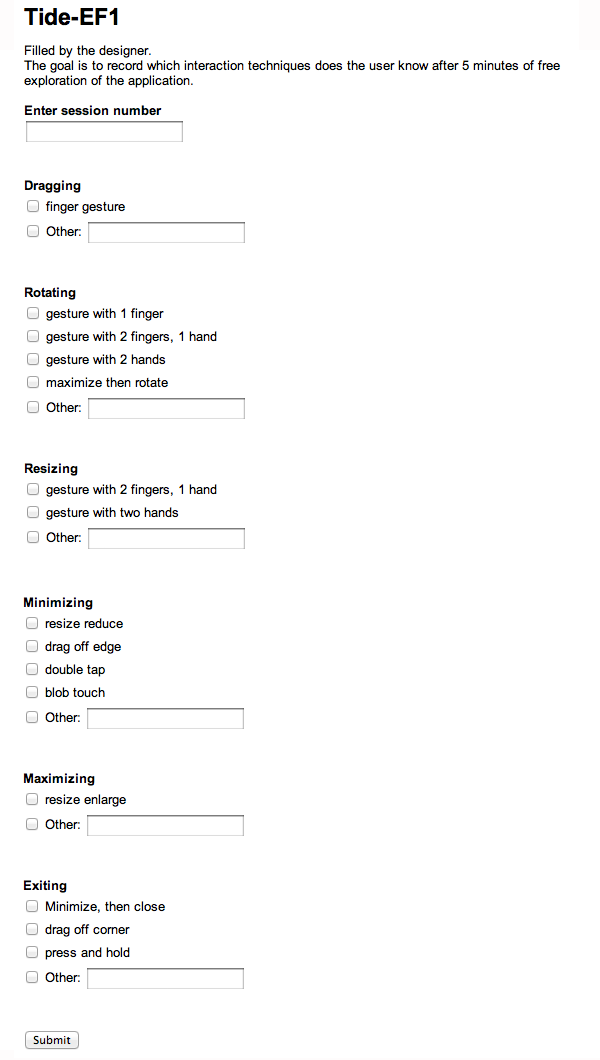
\includegraphics[width=0.7\textwidth]{images/evalform1}
    %\caption{TIDE: component diagram.}
    %\label{fig:overview}
\end{figure}

\begin{figure}[htb]
  \centering
    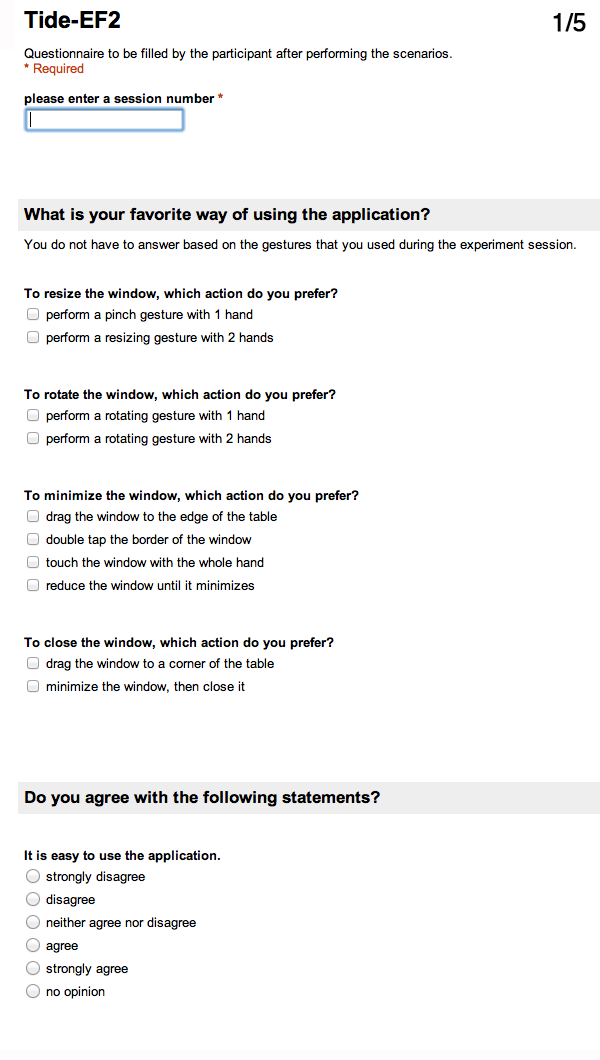
\includegraphics[width=0.8\textwidth]{images/evalform2a}
    %\caption{TIDE: component diagram.}
    %\label{fig:overview}
\end{figure}

\begin{figure}[htb]
  \centering
    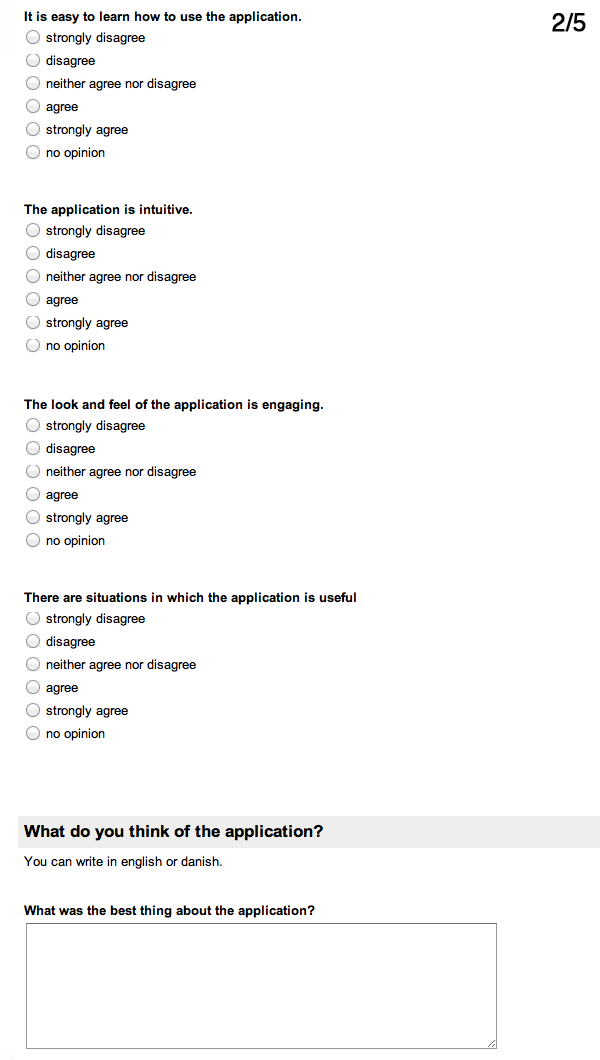
\includegraphics[width=0.8\textwidth]{images/evalform2b}
    %\caption{TIDE: component diagram.}
    %\label{fig:overview}
\end{figure}

\begin{figure}[htb]
  \centering
    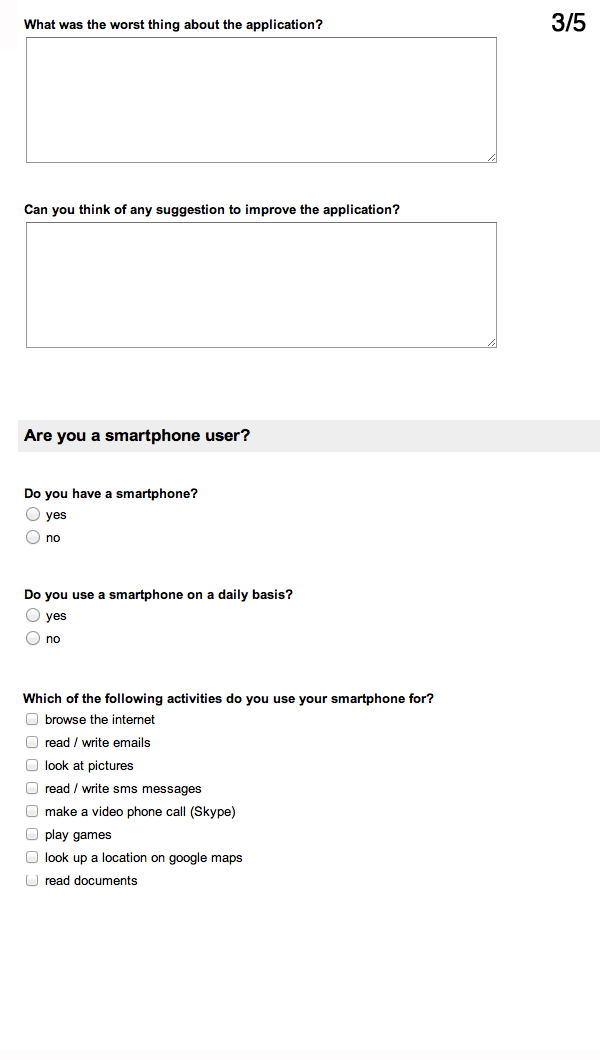
\includegraphics[width=0.8\textwidth]{images/evalform2c}
    %\caption{TIDE: component diagram.}
    %\label{fig:overview}
\end{figure}

\begin{figure}[htb]
  \centering
    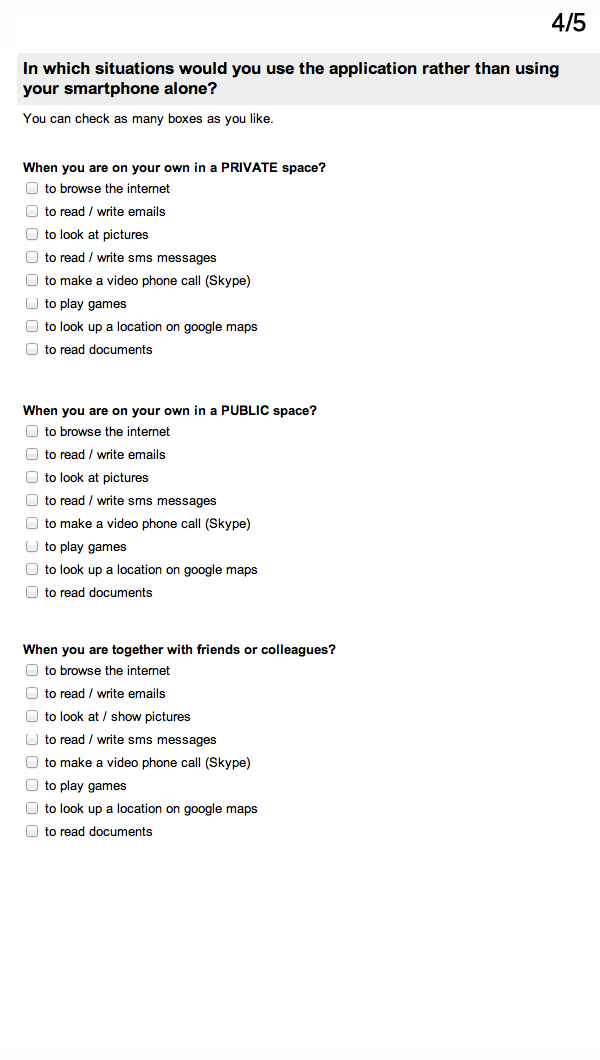
\includegraphics[width=0.8\textwidth]{images/evalform2d}
    %\caption{TIDE: component diagram.}
    %\label{fig:overview}
\end{figure}

\begin{figure}[htb]
  \centering
    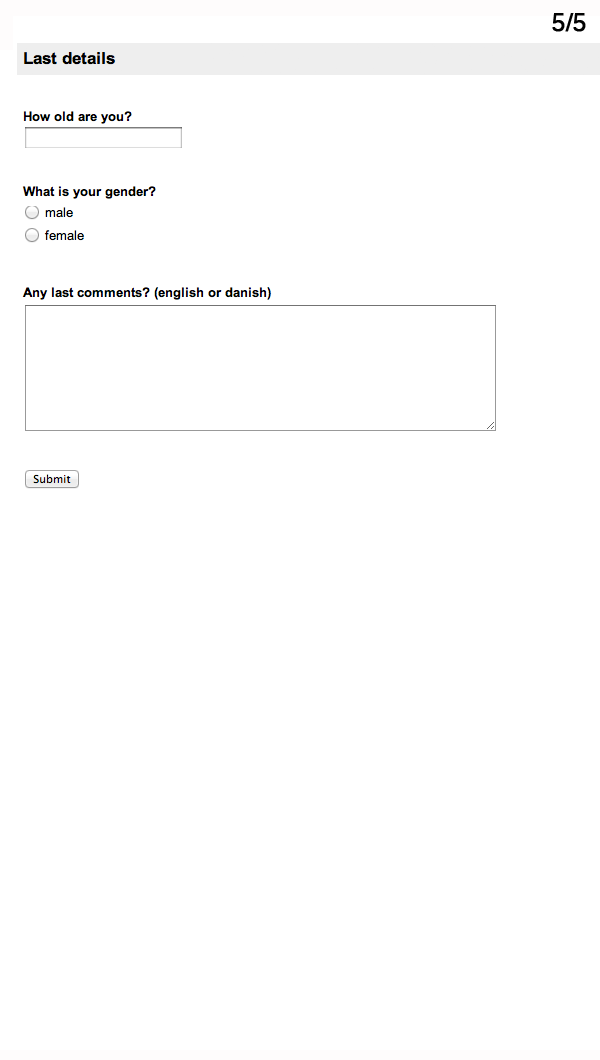
\includegraphics[width=0.8\textwidth]{images/evalform2e}
    %\caption{TIDE: component diagram.}
    %\label{fig:overview}
\end{figure}

%teaching phase for each primitive (5):
%1) ask them to do it
%	- do they know how to do it
%	- which technique do they use?
%2) ask them if they know of other technique
%- if yes, which? show?
%- if no, tell them. show?
%
%scenario phase:
%1) browsing:
%- pair Legend
%- look up sthg online: remote UI, dragging, resizing
%- shoe me sthg: rotating
%- hide stag from someone: minimizing/hiding
%
%2) gaming (designer is opponent)
%- pair iPhone
%- launch game: remote UI
%- resize to fullscreen (maximize)
%- exit
%
%questionnaire phase: google forms?
%= straightforward user satisfaction study
%- rate the experience: usable? engaging?
%- would you use such a system?
%- how intuitive is the system?
%
%
%LOGGING (user, session, command, action, timestamp)
%
%drag, resize, rotate = using active border
%
%maximize by size enlarge
%rotate when maximized
%
%minimize by drag to edge
%minimize by double tap
%minimize by blob touch
%minimize by size reduce
%
%close by minimize
%close by corner
%close by press and hold


\end{document}